%!TEX TS-program = xelatex
\documentclass[10pt,oneside,bigheadings,tablecaptionabove]{scrbook}
\usepackage{scrpage2}


\usepackage[a5paper,%landscape,
            top=0.5in,
            headheight=0.15in,
            headsep=0.25in,
            bottom=0.25in,
            left=0.25in,
            right=0.35in,
            footskip=0in,
            twocolumn=false]{geometry}
            
            
% tweak TOC formatting
\usepackage{tocloft}
\setlength{\cftsecnumwidth}{2em}            


\usepackage{fontspec}      % support opentype text fonts
\usepackage{unicode-math}  % support opentype math fonts
\usepackage{amsmath}
\usepackage{xltxtra}
%\usepackage[utf8]{inputenc}

\defaultfontfeatures{Scale=.92}
\setmainfont[Ligatures=TeX]{Lucida Bright OT}
\setsansfont[Ligatures=TeX]{Lucida Sans OT}
\setmonofont[Numbers=SlashedZero]{Lucida Sans Typewriter OT}
\setmathfont{Lucida Bright Math OT}
\setmathtt{Lucida Sans Typewriter OT}


\usepackage[square,numbers]{natbib}

\usepackage{bibentry}
\usepackage{microtype} 
\usepackage{graphicx}
\usepackage{booktabs}
\usepackage{units}
\usepackage{pdfpages}
\usepackage{paralist}
\usepackage{subfigure}
\usepackage[version=3]{mhchem} 
\usepackage{fancybox}
\usepackage{marginnote}
\renewcommand*{\marginfont}{\small\itshape} 

\usepackage[colorlinks=true,citecolor=blue,linkcolor=black]{hyperref}





\lstMakeShortInline|

\definecolor{boxfill}{gray}{0.975}
\definecolor{boxframe}{named}{gray}

\lstset{%
aboveskip=1ex,
xleftmargin=0.25em,
xrightmargin=0.25em,
breaklines=true,
basicstyle={\ttfamily \small},
breakatwhitespace=false,
showspaces=false,
showstringspaces=false
showtabs=false,
%keywordstyle=\color{DarkBlue}\bfseries,
%stringstyle=\color{DarkRed},
%commentstyle=\color{Olive}\itshape,
commentstyle=\color{gray!95}\itshape,
}


\lstnewenvironment{codeblock}[1][]
{\lstset{frame=single,
backgroundcolor=\color{boxfill},
rulecolor=\color{boxframe},
framesep=2.5pt,
framerule=0.5pt,
language=#1}}
{}

\lstnewenvironment{noindentcodeblock}[1][]
{\lstset{frame=single,
backgroundcolor=\color{boxfill},
rulecolor=\color{boxframe},
framesep=2.5pt,
framerule=0.5pt,
breakindent=0pt,
breakautoindent=false,
language=#1}}
{}

\lstnewenvironment{tinycode}[1][]
{\lstset{backgroundcolor=\color{boxfill},
basicstyle={\ttfamily \footnotesize},
language=#1}}
{}


\lstnewenvironment{code}
{\lstset{backgroundcolor=\color{boxfill}}}
{}

\lstnewenvironment{python}
{\lstset{language=python,backgroundcolor=\color{boxfill}}}
{}
\lstnewenvironment{bash}
{\lstset{language=bash,backgroundcolor=\color{boxfill}}}
{}
\lstnewenvironment{R}
{\lstset{language=R,backgroundcolor=\color{boxfill}}}
{}



% Assignment box environment

\usepackage{chngcntr}  % provides \counterwithin
\newcounter{assignnum}
\counterwithin{assignnum}{chapter}
\setcounter{assignnum}{1}
\newenvironment{assignment}{%
\tcolorbox[colback=DarkRed!5,colframe=DarkRed!50,fonttitle=\sffamily\bfseries,title={Assignment \stepcounter{assignnum}\theassignnum},fontupper=\small,fontlower=\small,boxrule=0.1pt,left=2mm,right=2mm]}%
{\endtcolorbox}


%\usepackage[small,compact]{titlesec}

% for figures
\usepackage[margin=10pt,font=small]{caption}
\usepackage{subcaption}
\usepackage{graphicx}
\usepackage[usenames, dvipsnames]{xcolor}


% Assignment box environment

\usepackage{fancybox}
\usepackage{fancyvrb}

\newcounter{assign_num}
\setcounter{assign_num}{1}
\newenvironment{assignment}%
{\begin{Sbox}\begin{minipage}{6in}%
\textbf{Assignment \arabic{assign_num}\stepcounter{assign_num}}:}% 
{\end{minipage}\end{Sbox}\shadowbox{\TheSbox}}


% Comment box environment

\newenvironment{commentbox}%
{\setlength{\fboxsep}{15pt}%
\begin{Sbox}%
\begin{minipage}{6in}%
\sffamily \vspace*{1ex}%
\textbf{\large Comments}\vspace*{0.5ex}\color{red}\\}% 
{\vspace*{0.5ex}%
\end{minipage}\end{Sbox}\ovalbox{\TheSbox}}

\newenvironment{comment}[1]{\vspace*{2ex}\sffamily \color{red} #1}{\vspace*{2ex}}



%% Fancy syntax coloring via pygments
\usepackage{minted}
\usemintedstyle{bw}

\definecolor{bg}{rgb}{0.96,0.96,0.96}

\newenvironment{Rcode}
{\VerbatimEnvironment
 \begin{minted}[xleftmargin=1em, baselinestretch=0.88]{r}}%
{\end{minted}}


\newenvironment{Pcode}
{\VerbatimEnvironment
 \begin{minted}[xleftmargin=1em,baselinestretch=0.88]{python}}%
{\end{minted}}

\newenvironment{Code}[1]
{\VerbatimEnvironment
 \begin{minted}[framesep=0.5em,xleftmargin=1em]{#1}}%
{\end{minted}}


\newenvironment{PageCode}[1]
{\VerbatimEnvironment
 \begin{minted}[frame=single, framerule=1.5pt,framesep=0.5em,xleftmargin=1em]{#1}}%
{\end{minted}}

% \DefineShortVerb{\|} 
% \everymath{\UndefineShortVerb{\|}\vert}


\newcommand{\Species}[1]{{\rmfamily \itshape #1}}

% Math related macros
\newcommand{\Real}{\ensuremath{\mathbb{R}}}
\newcommand{\RealN}{\ensuremath{\mathbb{R}^n}}
\newcommand{\RealP}{\ensuremath{\mathbb{R}^p}}
\newcommand{\Mtx}[1]{\ensuremath{\mathbf{#1}}}
\newcommand{\Inv}[1]{\ensuremath{#1^{-1}}}
\newcommand{\InvMtx}[1]{\ensuremath{\mathbf{#1}^{-1}}}
\newcommand{\Red}[1]{\textcolor{red}{#1}}
\newcommand{\PsInv}[1]{\ensuremath{\mathbf{#1}^{+}}}




% Hyperref should be the last package
\usepackage{hyperref}
\hypersetup{
colorlinks=true
}


\definecolor{Dark}{gray}{.2}
\definecolor{MedDark}{gray}{.4}
\definecolor{Medium}{gray}{.6}
\definecolor{Light}{gray}{.8}

\newlength{\tpheight}\setlength{\tpheight}{0.9\textheight}
\newlength{\txtheight}\setlength{\txtheight}{0.9\tpheight}
\newlength{\tpwidth}\setlength{\tpwidth}{0.9\textwidth}
\newlength{\txtwidth}\setlength{\txtwidth}{0.9\tpwidth}
\newlength{\drop}

\newcommand*{\titleLL}{\begingroup% Lost Languages
\drop=0.1\txtheight
\fboxsep 0.5\baselineskip
\sffamily
\vspace*{\drop}
\centering
{\textcolor{DarkRed}{\Huge Bio 723}}\par
\vspace{0.5\drop}
\colorbox{black}{\textcolor{white}{\normalfont\itshape\Large Scientific Computing for Biologists}}\par
\vspace{\drop}
{\textcolor{black}{\Large R Programming Workbook}}\par

\vspace{\drop}
{\Large Paul M. Magwene}\par
\vfill
{\large Fall 2014}\par
\vspace*{\drop}
\endgroup}



\usepackage[colorlinks=true,
            citecolor=blue,
            linkcolor=black,
            breaklinks=true,
            linktocpage]{hyperref}


\usepackage[capitalize]{cleveref} % should always be loaded after hyperref


%% Document
\begin{document}
\savegeometry{oldgeom}


\clearscrheadfoot
\pagestyle{scrheadings}
\newgeometry{twocolumn=false,a5paper,%landscape,
            top=0.5in,
            headheight=0.15in,
            headsep=0.25in,
            bottom=0.25in,
            left=0.2in,
            right=0.2in,
            footskip=0in}

\titleLL
\clearpage
%\restoregeometry
\loadgeometry{oldgeom}


\tableofcontents
\clearpage


\clearscrheadfoot
\setheadcolor{DarkRed!3}
\ihead{\tikzhead\headmark}
\ohead{\pagemark}
\setkomafont{pagehead}{\normalfont\sffamily}
\setkomafont{pagenumber}{\normalfont\sffamily}
\pagestyle{scrheadings}
\renewcommand*{\chapterpagestyle}{scrheadings}


\chapter{Getting your feet wet with R}


\section{Getting Acquainted with R}

\subsection{Installing R}


The R website is at \url{http://www.r-project.org/}. I recommend that you spend a few minutes checking out the resources, documentation, and links on this page.   Download the appropriate R installer for your computer from the Comprehensive R Archive Network (CRAN). A direct link can be found at: \url{http://cran.stat.ucla.edu/}. As of mid August 2012 the latest R release is verison 2.15.1.

The R installer will install appropriate icons under the |Start Menu| (Windows) or |Applications| Folder (OS X). On OS X it will install two icons -- ``R" and ``R64", corresponding to 32-bit and 64-bit versions of the executable.  The 64 bit version, which allows access to much larger amounts of your comptuer's RAM, is suitable for dealing with very large data sets. 


\subsection{Starting and R Interactive Session}

 The \OSX and Windows version of R provide a simple GUI
interface for using R in interactive mode. When you start up the R GUI you'll be
presented with a single window, the R console. See the your textbook, The Art of R Programming (AoRP) for a discussion of the difference between R's interactive and batch modes.

\subsection{Accessing the Help System on R}

R comes with fairly extensive documentation and a simple help system. You can
access HTML versions of R documentation under the Help menu in the GUI. The
HTML documentation also includes information on any packages you've installed.
Take a few minutes to browse through the R HTML documentation.

The help system can be invoked from the console itself using the
|help| function or the |?| operator.
%
\begin{R}
> help(length)
> ?length
> ?log
\end{R}
%
What if you don't know the name of the function you want? You can use
the |help.search()| function.
%
\begin{R}
> help.search("log")
\end{R}
%
In this case |help.search("log")| returns all the functions with
the string `log' in them. For more on |help.search| type
|?help.search|. Other useful help related functions include
|apropos()| and |example()|.

\subsection{Navigating Directories in R}

When you start the R environment your `working directory' (i.e.~the
directory on your computer's file system that R currently `sees')
defaults to a specific directory. On Windows this is usually the same
directory that R is installed in, on \OSX it is typically your home
directory. Here are examples showing how you can get information about
your working directory and change your working directory.
%
\begin{R}
> getwd()
[1] "/Users/pmagwene"
> setwd("/Users")
> getwd()
[1] "/Users"
\end{R}
%
Note that on Windows you can change your working directory by using the
|Change dir...| item under the |File| menu, while the corresponding item is found under the |Misc| menu on \OSX.

To get a list of the file in your current working directory use the
|list.files()| function.
%
\begin{R}
> list.files()
[1] "Shared" "pmagwene"
\end{R}



\subsection{Using R as a Calculator}

The simplest way to use R is as a fancy calculator.
%
\begin{R}
> 10 + 2 # addition
[1] 12
> 10 - 2 # subtraction
[1] 8
> 10 * 2 # multiplication
[1] 20
> 10 / 2 # division
[1] 5
> 10 ^ 2 # exponentiation
[1] 100
> 10 ** 2 # alternate exponentiation
[1] 100
> sqrt(10) # square root
[1] 3.162278
> 10 ^ 0.5 # same as square root
[1] 3.162278
> exp(1) # exponential function
[1] 2.718282
> 3.14 * 2.5^2
[1] 19.625
> pi * 2.5^2 # R knows about some constants such as Pi
[1] 19.63495
> cos(pi/3)
[1] 0.5
> sin(pi/3)
[1] 0.8660254
> log(10)
[1] 2.302585
> log10(10) # log base 10
[1] 1
> log2(10) # log base 2
[1] 3.321928
> (10 + 2)/(4-5)
[1] -12
> (10 + 2)/4-5 # compare the answer to the above
[1] -2
\end{R}
%
Be aware that certain operators have precedence over others. For example
multiplication and division have higher precedence than addition and
subtraction. Use parentheses to disambiguate potentially confusing
statements.

\begin{R}
> sqrt(pi)
[1] 1.772454
> sqrt(-1)
[1] NaN
Warning message:
NaNs produced in: sqrt(-1)
> sqrt(-1+0i)
[1] 0+1i
\end{R}
%
What happened when you tried to calculate |sqrt(-1)|?, -1 is
treated as a real number and since square roots are undefined for the
negative reals, R produced a warning message and returned a special
value called |NaN| (Not a Number). Note that square roots of
negative complex numbers are well defined so |sqrt(-1+0i)|
works fine.
%
\begin{R}
> 1/0
[1] Inf
\end{R}
Division by zero produces an object that represents infinite numbers.

\subsection{Comparison Operators}

You've already been introduced to the most commonly used arithmetic
operators. Also useful are the comparison operators:
%
\begin{R}
> 10 < 9  # less than
[1] FALSE
> 10 > 9  # greater than
[1] TRUE
> 10 <= (5 * 2) # less than or equal to
[1] TRUE
> 10 >= pi # greater than or equal to
[1] TRUE
> 10 == 10 # equals
[1] TRUE
> 10 != 10 # does not equal
[1] FALSE
> 10 == (sqrt(10)^2) # Surprised by the result? See below.
[1] FALSE
> 4 == (sqrt(4)^2) # Even more confused?
[1] TRUE
\end{R}
%
Comparisons return boolean values. Be careful to distinguish between
|==| (tests equality) and |=| (the alternative
assignment operator equivalent to |<-|).

How about the last two statement comparing two values to the square of
their square roots? Mathematically we know that both
$(\sqrt{10})^2 = 10$ and $(\sqrt{4})^2 = 4$ are true statements. Why
does R tell us the first statement is false? What we're running into
here are the limits of computer precision. A computer can't represent
$\sqrt 10$ exactly, whereas $\sqrt 4$ can be exactly represented.
Precision in numerical computing is a complex subject and beyond the
scope of this course. Later in the course we'll discuss some ways of
implementing sanity checks to avoid situations like that illustrated
above.

\subsection{Working with Vectors in R}

Vectors are the core data structure in R. Vectors store an ordered list of items all of the same type. Learning to compute effectively with vectors and one of the keys to efficient R programming.  Vectors in R always have a length (accessed with the |length()| function) and a type (accessed with the |typeof()| function).  

The simplest way to create a vector at the interactive prompt is to use the |c()| function, which is short hand for `combine' or `concatenate'.

\begin{R}
> x <- c(2,4,6,8)
[1] "double"
> length(x)
[1] 4
> y <- c('joe','bob','fred')
> typeof(y)
[1] "character"
> length(y)
[1] 3
> z <- c() # empty vector
> length(z)
[1] 0
> typeof(z)
[1] "NULL"
\end{R}

You can also use |c()| to concatenate two or more vectors together.
%
\begin{R}
> v <- c(1,3,5,7)
> w <- c(-1, -2, -3)
> vwx <- c(v,w,x)
> vwx
 [1]  1  3  5  7 -1 -2 -3  2  4  6  8
\end{R}

\subsubsection{Vector Arithmetic and Comparison}

The basic R arithmetic operations work on vectors as well as on
single numbers (in fact single numbers \emph{are} vectors).
%
\begin{R}
> x <- c(2, 4, 6, 8, 10)
> x * 2
[1]  4  8 12 16 20
> x * pi
[1]  6.283185 12.566371 18.849556 25.132741 31.415927
> y <- c(0, 1, 3, 5, 9)
> x + y
[1]  2  5  9 13 19
> x * y
[1]  0  4 18 40 90
> x/y
[1]      Inf 4.000000 2.000000 1.600000 1.111111
> z <- c(1, 4, 7, 11)
> x + z
[1]  3  8 13 19 11
Warning message:
longer object length
        is not a multiple of shorter object length in: x + z
\end{R}
%
When vectors are not of the same length R `recycles' the elements of the
shorter vector to make the lengths conform. In the example above
|z| was treated as if it was the vector |(1, 4, 7, 11, 1)|.


The comparison operators also work on vectors as shown below.
Comparisons involving vectors return vectors of booleans.
%
\begin{R}
> x > 5
[1] FALSE FALSE  TRUE  TRUE  TRUE
> x != 4
[1]  TRUE FALSE  TRUE  TRUE  TRUE
\end{R}

If you try and apply arithmetic operations to non-numeric vectors, R will warn you of the error of your ways:
%
\begin{R}
> w <- c('foo', 'bar', 'baz', 'qux')
> w**2
Error in w^2 : non-numeric argument to binary operator
\end{R}
%
Note, however that the comparison operators can work with non-numeric vectors. The results you get will depend on the type of the elements in the vector.
%
\begin{R}
>  w == 'bar'
[1] FALSE  TRUE FALSE FALSE
> w < 'cat'
[1] FALSE  TRUE  TRUE FALSE
\end{R}


\subsubsection{Indexing Vectors}

For a vector of length $n$, we can access the elements by the indices $1
\ldots n$. We say that R vectors (and other data structures like lists) are `one-indexed'. Many other programming languages, such as Python, C, and Java, use zero-indexing where the elements of a data structure are accessed by the indices $0 \ldots n-1$. Indexing errors are a common source of bugs. When moving back and forth between different programming languages keep the appropriate indexing straight!

Trying to access an element beyond these limits returns a special
constant called |NA| (Not Available) that indicates missing or non-existent
values.
%
\begin{R}
> x <- c(2, 4, 6, 8, 10)
> length(x)
[1] 5
> x[1]
[1] 2
> x[4]
[1] 8
> x[6]
[1] NA
> x[-1]
[1]  4  6  8 10
> x[c(3,5)]
[1]  6 10
\end{R}
%
Negative indices are used to exclude particular elements. |x[-1]| returns all
elements of |x| except the first. You can get multiple elements of a vector by
indexing by another vector. In the example above |x[c(3,5)]| returns the third
and fifth element of |x|.

\subsubsection{Combining Indexing and Comparison}

A very powerful feature of R is the ability to combine the comparison
operators with indexing. This facilitates data filtering and subsetting.
Some examples:
%
\begin{R}
> x <- c(2, 4, 6, 8, 10)
> x[x > 5]
[1]  6  8 10
> x[x < 4 | x > 6]
[1]  2  8 10
\end{R}
%

In the first example we retrieved all the elements of |x| that are larger than
5 (read as `x where x is greater than 5'). In the second example we retrieved
those elements of |x| that were smaller than four \emph{or} greater than six.
The symbol \lstinline!|! is the `logical or' operator. Other logical operators
include |&| (`logical and' or `intersection') and |!| (negation). Combining
indexing and comparison is a powerful concept and one you'll probably find
useful for analyzing your own data.

\subsubsection{Generating Regular Sequences}

Creating sequences of numbers that are separated by a specified value or
that follow a particular patterns turns out to be a common task in
programming. R has some built-in operators and functions to simplify
this task.
%
\begin{R}
> s <- 1:10
> s
 [1]  1  2  3  4  5  6  7  8  9 10
> s <- 10:1
> s
 [1] 10  9  8  7  6  5  4  3  2  1
> s <- seq(0.5,1.5,by=0.1)
> s
 [1] 0.5 0.6 0.7 0.8 0.9 1.0 1.1 1.2 1.3 1.4 1.5
# 'by' is the 3rd argument so you don't have to specify it
> s <- seq(0.5, 1.5, 0.33)
> s
[1] 0.50 0.83 1.16 1.49
\end{R}

|rep()| is another way to generate patterned data.
%
\begin{R}
> rep(c("Male","Female"),3)
[1] "Male"   "Female" "Male"   "Female" "Male"   "Female"
> rep(c(T,T, F),2)
[1]  TRUE  TRUE FALSE  TRUE  TRUE FALSE
\end{R}


\subsection{Some Useful Functions}

You've already seem a number of functions (|c()|, |length()|, |sin()|,
|log|, |length()|, etc). Functions are called by
invoking the function name followed by parentheses containing zero or
more \emph{arguments} to the function. Arguments can include the data
the function operates on as well as settings for function parameter
values. We'll discuss function arguments in greater detail below.

\subsubsection{Creating longer vectors}

For vectors of more than 10 or so elements it gets tiresome and error
prone to create vectors using |c()|. For medium length vectors
the |scan()| function is very useful.
%
\begin{R}
> test.scores <- scan()
1: 98 92 78 65 52 59 75 77 84 31 83 72 59 69 71 66
17:
Read 16 items
> test.scores
 [1] 98 92 78 65 52 59 75 77 84 31 83 72 59 69 71 66
\end{R}
%
When you invoke |scan()| without any arguments the function
will read in a list of values separated by white space (usually spaces
or tabs). Values are read until |scan()| encounters a blank
line or the end of file (EOF) signal (platform dependent). We'll see how to read in data from files below.

Note that we created a variable with the name |test.scores|.
If you have previous programming experience you might be surprised that
this works. Unlike most languages, R allows you to use periods in
variable names. Descriptive variable names generally improve readability
but they can also become cumbersome (e.g.
|my.long.and.obnoxious.variable.name|). As a general rule of
thumb use short variable names when working at the interpreter and more
descriptive variable names in functions.

\subsubsection{Useful Numerical Functions}

Let's introduce some additional numerical functions that are useful for
operating on vectors.
%
\begin{R}
> sum(test.scores)
[1] 1131
> min(test.scores)
[1] 31
> max(test.scores)
[1] 98
> range(test.scores) # min,max returned as a vec of len 2
[1] 31 98
> sorted.scores <- sort(test.scores)
> sorted.scores
 [1] 31 52 59 59 65 66 69 71 72 75 77 78 83 84 92 98
> w <- c(-1, 2, -3, 3)
> abs(w) # absolute value function
\end{R}

\subsection{Function Arguments in R}

Function arguments can specify the data that a function operates on or
parameters that the function uses. Some arguments are required, while
others are optional and are assigned default values if not specified.

Take for example the |log()| function. If you examine the help
file for the |log()| function (type |?log| now) you'll see that it takes two
arguments, refered to as `|x|' and `|base|'. The
argument |x| represents the numeric vector you pass to the
function and is a required argument (see what happens when you type
|log()| without giving an argument). The argument
|base| is optional. By default the value of |base|
is $e = 2.71828\ldots$. Therefore by default the |log()|
function returns natural logarithms. If you want logarithms to a
different base you can change the |base| argument as in the
following examples:
%
\begin{R}
> log(2) # log of 2, base e
[1] 0.6931472
> log(2,2) # log of 2, base 2
[1] 1
> log(2, 4) # log of 2, base 4
[1] 0.5
\end{R}

Because base 2 and base 10 logarithms are fairly commonly used, there are convenient aliases for calling log with these bases.
%
\begin{R}
> log2(8)
[1] 3
> log10(100)
[1] 2    
\end{R}

\subsection{Lists in R}

R lists are like vectors, but unlike a vector where all the elements are of the same type, the elements of a list can have arbitrary types (even other lists). 
\begin{R}
> l <- list('Bob', pi, 10, c(2,4,6,8))
\end{R}
Indexing of lists is different than indexing of vectors.  Double brackets (|x[[i]]|) return the element at index $i$, single bracket return a list containing the element at index $i$.
\begin{R}
> l[1] # single brackets
[[1]]
[1] "Bob"

> l[[1]] # double brackets
[1] "Bob"
> typeof(l[1])
[1] "list"
> typeof(l[[1]])
[1] "character"
\end{R}
The elements of a list can be given names, and those names objects can be accessed using the |$| operator. You can retrieve the names associated with a list using the |names()| function.
\begin{R}
> l <- list(name='Bob', age=27, years.in.school=10)
> l
$name
[1] "Bob"

$age
[1] 27

$years.in.school
[1] 10

> l$years.in.school
[1] 10
> l$name
[1] "Bob"
> names(l)
[1] "name"            "age"             "years.in.school"    
\end{R}


\subsection{Simple Input in R}

The \lstinline!c()! and \lstinline!scan()! functions are fine for
creating small to medium vectors at the interpreter, but eventually
you'll want to start manipulating larger collections of data. There are
a variety of functions in R for retrieving data from files.

The most convenient file format to work with are tab delimited text
files. Text files have the advantage that they are human readable and
are easily shared across different platforms. If you get in the habit of
archiving data as text files you'll never find yourself in a situation
where you're unable to retrieve important data because the binary data
format has changed between versions of a program.

\subsection{Using \lstinline!scan()! to input data}

\lstinline!scan()! itself can be used to read data out of a file.
Download the file \lstinline!algae.txt! from the class website and try
the following (after changing your working directory):

\begin{R}
> algae <- scan('algae.txt')
Read 12 items
> algae
 [1] 0.530 0.183 0.603 0.994 0.708 0.006 0.867 0.059 0.349 0.699 0.983 0.100
\end{R}
One of the things to be aware of when using \lstinline!scan()! is that
if the data type contained in the file can not be coerced to doubles
than you must specify the data type using the \lstinline!what! argument.
The \lstinline!what! argument is also used to enable the use of
\lstinline!scan()! with columnar data. Download \lstinline!algae2.txt!
and try the following:

\begin{R}
> algae.table <- scan('algae2.txt', what=list('',double(0)))
                        # note use of list argument to what
> algae.table

> algae.table
[[1]]
 [1] "Jan" "Feb" "Mar" "Apr" "May" "Jun" "Jul" "Aug" "Sep" "Oct" "Nov"
[12] "Dec"

[[2]]
 [1] 0.530 0.183 0.603 0.994 0.708 0.006 0.867 0.059 0.349 0.699 0.983
[12] 0.100

> algae.table[[1]]
 [1] "Jan" "Feb" "Mar" "Apr" "May" "Jun" "Jul" "Aug" "Sep" "Oct" "Nov"
[12] "Dec"
> algae.table[[2]]
 [1] 0.530 0.183 0.603 0.994 0.708 0.006 0.867 0.059 0.349 0.699 0.983
[12] 0.100
\end{R}
Use help to learn more about \lstinline!scan()!.

\subsection{Using \lstinline!read.table()! to input data}

\lstinline!read.table()! (and it's derivates - see the help file)
provides a more convenient interface for reading tabular data. Download the \lstinline|turtles.txt| data set from the class wiki.  The data in \lstinline|turtles.txt| are a set of linear measurements representing dimensions of the carapace (upper shell) of painted turtles (\textit{Chrysemys picta}), as reported in Jolicoeur and Mosimmann, 1960; Growth 24: 339-354.

Using the
file \lstinline!turtles.txt!:

\begin{R}
> turtles <- read.table('turtles.txt', header=T)
> turtles
   sex length width height
1    f     98    81     38
2    f    103    84     38
3    f    103    86     42
  # output truncated
> names(turtles)
[1] "sex"    "length" "width"  "height"
> length(turtles)
[1] 4
> length(turtles$sex)
[1] 48
\end{R}
What kind of data structure is \lstinline!turtles!? What happens when
you call the \lstinline!read.table()! function without specifying the
argument \lstinline!header=T!?

You'll be using the \lstinline!read.table()}!function frequently. Spend
some time reading the documentation and playing around with different
argument values (for example, try and figure out how to specify
different column names on input).

Note: \lstinline!read.table()! is more convenient but \lstinline!scan()!
is more efficient for large files. See the R documentation for more
info.

\subsection{Basic Statistical Functions in R}

There are a wealth of statistical functions built into R. Let's start to
put these to use.

If you wanted to know the mean carapace width of turtles in your sample
you could calculate this simply as follows:

\begin{R}
> sum(turtles$width)/length(turtles$width)
[1] 95.4375
\end{R}
Of course R has a built in \lstinline!mean()! function.

\begin{R}
mean(turtles$width) [1] 95.4375
\end{R}
One of the advantages of the built in \lstinline!mean()! function is
that it knows how to operate on lists as well as vectors:

\begin{R}
> mean(turtles)
      sex    length     width    height
       NA 124.68750  95.43750  46.33333
Warning message:
argument is not numeric or logical: returning NA in: mean.default(X[[1]], ...)
\end{R}
Can you figure out why the above produced a warning message? Let's take
a look at some more standard statistical functions:

\begin{R}
> min(turtles$width)
[1] 74
> max(turtles$width)
[1] 132
> range(turtles$width)
[1]  74 132
> median(turtles$width)
[1] 93
> summary(turtles$width)
   Min. 1st Qu.  Median    Mean 3rd Qu.    Max.
  74.00   86.00   93.00   95.44  102.00  132.00
> var(turtles$width) # variance
[1] 160.6769
> sd(turtles$width)  # standard deviation
[1] 12.67584
\end{R}


% \subsection{Simple Plots in R}

% One of the advantages of R is it's ability to produce a variety of plots
% and statistical graphics. Try out the following:

% \begin{R}
% > hist(turtles$width)  # histogram plot
% > hist(turtles$width,10) # produces a histogram with 10 bins
% > hist(turtles$width,breaks=10, xlab="Carapace Width", probability=T)
% > boxplot(turtles$width) # simple box plot
% # a fancy box plot showing multiple variables
% > boxplot(list(turtles$length, turtles$width,  turtles$height),
% +        names=c("Carapace\nLength","Carapace\nWidth","Carapace\nHeight"),
% +        ylab="millimeters")
% > title("Turtle Shell Variables")
% > plot(turtles$length, turtles$width)
% # how does this differ from the plot above?
% > plot(turtles$length ~ turtles$width)
% > plot(turtles$length, turtles$width,
% +      xlab="Carapace Length(mm)", ylab="Carapace Width(mm)")
% > title("Relationship Between\nLength and Width")
% \end{R}


% To get a sense of some of the graphical power of R try the
% \lstinline!demo()! function:
% %
% \begin{R}
% > demo(graphics)
% \end{R}


\section{Exploring Univariate Distributions in R}

\subsection{Histograms}

One of the most common ways to examine a the distribution of
observations for a single variable is to use a histogram. The
\lstinline!hist()! function creates simple histograms in R.

\begin{R}
> hist(turtles$length) # create histogram with fxn defaults
> ?hist # check out the documentation on hist
\end{R}
Note that by default the \lstinline!hist()! function plots the
frequencies in each bin. If you want the probability densities instead
set the argument \lstinline!freq=FALSE!.
%
\begin{R}
> hist(turtles$length,freq=F) # y-axis gives probability density
\end{R}
Here's some other ways to fine tune a histogram in R.

\begin{R}
> hist(turtles$length, breaks=12) # use 12 bins
> mybreaks = seq(85,185,8)
> hist(turtles$length, breaks=mybreaks) # specify bin boundaries
> hist(turtles$length, breaks=mybreaks, col='red') # fill the bins with red
\end{R}

\subsection{Density Plots}

One of the problems with histograms is that they can be very sensitive
to the size of the bins and the break points used. This is due to the
discretization inherent in a histogram. A `density plot' or `density
trace' is a continuous estimate of a probability distribution from a set
of observations. Because it is continuous it doesn't suffer from the
same sensitivity to bin sizes and break points. One way to think about a
density plot is as the histogram you'd get if you averaged many
individual histograms each with slightly different breakpoints.
%
\begin{R}
> d <- density(turtles$length)
> plot(d)
\end{R}
%
A density plot isn't entirely parameter free -- the parameter you should
be most aware of is the `smoothing bandwidth'.

\begin{R}
> d <- density(turtles$length) # let R pick the bandwidth
> plot(d,ylim=c(0,0.020)) # gives ourselves some extra headroom on y-axis
> d2 <- density(turtles$length, bw=5) # specify bandwidth
> lines(d2, col='red') # use lines to draw over previous plot
\end{R}
The bandwidth determines the standard deviation of the `kernel' that is
used to calculate the density plot. There are a number of different
types of kernels you can use; a Gaussian kernel is the R default and is
the most common choice. See the documentation for more info.

The \lstinline!lattice! package is an R library that makes it easier to
create graphics that show conditional distributions. Here's how to
create a simple density plot using the \lstinline!lattice! package.

\begin{R}
> library(lattice)
> densityplot(turtles$length) # densityplot defined in lattice
\end{R}
Notice how by default the \lstinline!lattice! package also drew points
representing the observations along the x-axis. These points have been
`jittered' meaning they've been randomly shifted by a small amount so
that overlapping points don't completely hide each other. We could have
produced a similar plot, without the lattice package, as so:

\begin{R}
> d <- density(turtles$length)
> plot(d)
> nobs <- length(turtles$length)
> points(jitter(turtles$length), rep(0,nobs))
\end{R}
Notice that in our version we only jittered the points along the x-axis.
You can also combine a histogram and density trace, like so:

\begin{R}
> hist(turtles$length, 10, xlab='Carapace Length (mm)',freq=F)
> d <- density(turtles$length)
> lines(d, col='red', lwd=2) # red lines, with pixel width 2
\end{R}
Notice the use of the \lstinline!freq=F! argument to scale the histogram
bars in terms of probability density.

Finally, let's some of the features of \lstinline!lattice! to produce
density plots for the `length' variable of the turtle data set,
conditional on sex of the specimen.

\begin{R}
> densityplot(~length | sex, data = turtles)
\end{R}
There are a number of new concepts here. The first is that we used what
is called a `formula' to specify what to plot. In this case the formula
can be read as `length conditional on sex'. We'll be using formulas in
several other contexts and we discuss them at greater length below. The
\lstinline!data! argument allows us to specify a data frame or list so
that we don't always have to write arguments like
\lstinline!turtles$length! or \lstinline!turtles$sex! which can get a
bit tedious.

\subsection{Box Plots}

Another common tool for depicting a univariate distribution is a `box
plot' (sometimes called a box-and-whisker plot). A standard box plot
depicts five useful features of a set of observations: the median
(center most line), the upper and lower quartiles (top and bottom of the
box), and the minimum and maximum observations (ends of the whiskers).

\begin{figure}[htbp]
\centering
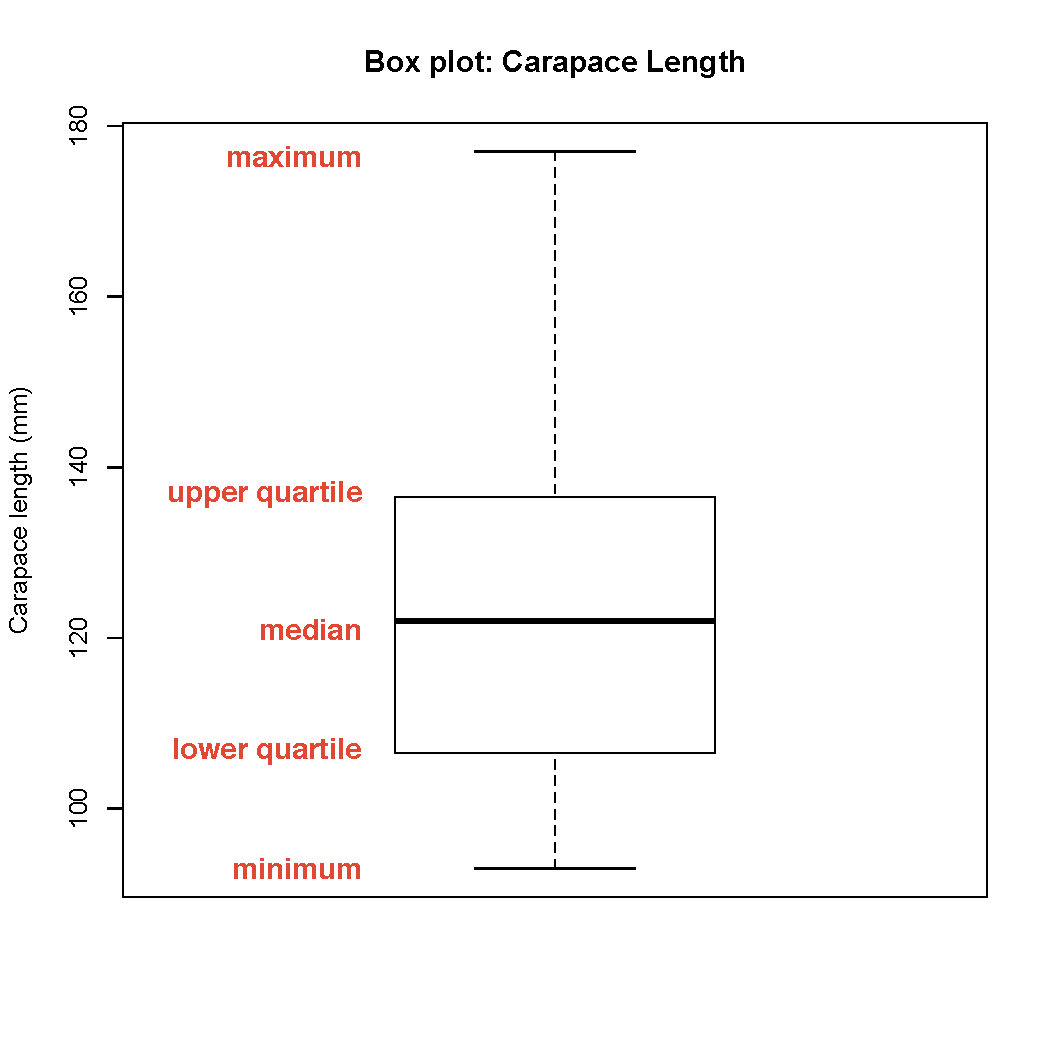
\includegraphics[width=0.5\columnwidth]{./figures/hands-on2/boxplot-labeled.pdf}
\caption{A box plot represents a five number summary of a set of
observations.}
\end{figure}

There are many variants on box plots, particularly with respect to the
`whiskers'. It's always a good idea to be explicit about what a box plot
you've created depicts.

Here's how to create box plots using the standard R functions as well as
the lattice package:

\begin{R}
> boxplot(turtles$length)
> boxplot(turtles$length, col='darkred', horizontal=T) # horizontal version
> title(main = 'Box plot: Carapace Length', ylab = 'Carapace length (mm)')
> bwplot(~length,data=turtles) # using the bwplot function from lattice
\end{R}
Note how we used the \lstinline!title()! function to change the axis
labels and add a plot title.

\paragraph{Historical note}

-- The box plot is one of many inventions of the statistician John W.
Tukey. Tukey made many contributions to the field of statistics and
computer science, particularly in the areas of graphical representations
of data and exploratory data analysis.

\subsection{Bean Plots}

My personal favorite way to depict univariate distributions is called a
`beanplot'. Beanplots combine features of density plots and boxplots and
provide information rich graphical summaries of single variables. The
standard features in a beanplot include the individual observations
(depicted as lines), the density trace estimated from the observations,
the mean of the observations, and in the case of multiple beanplots an
overall mean.

\begin{figure}[htbp]
\centering
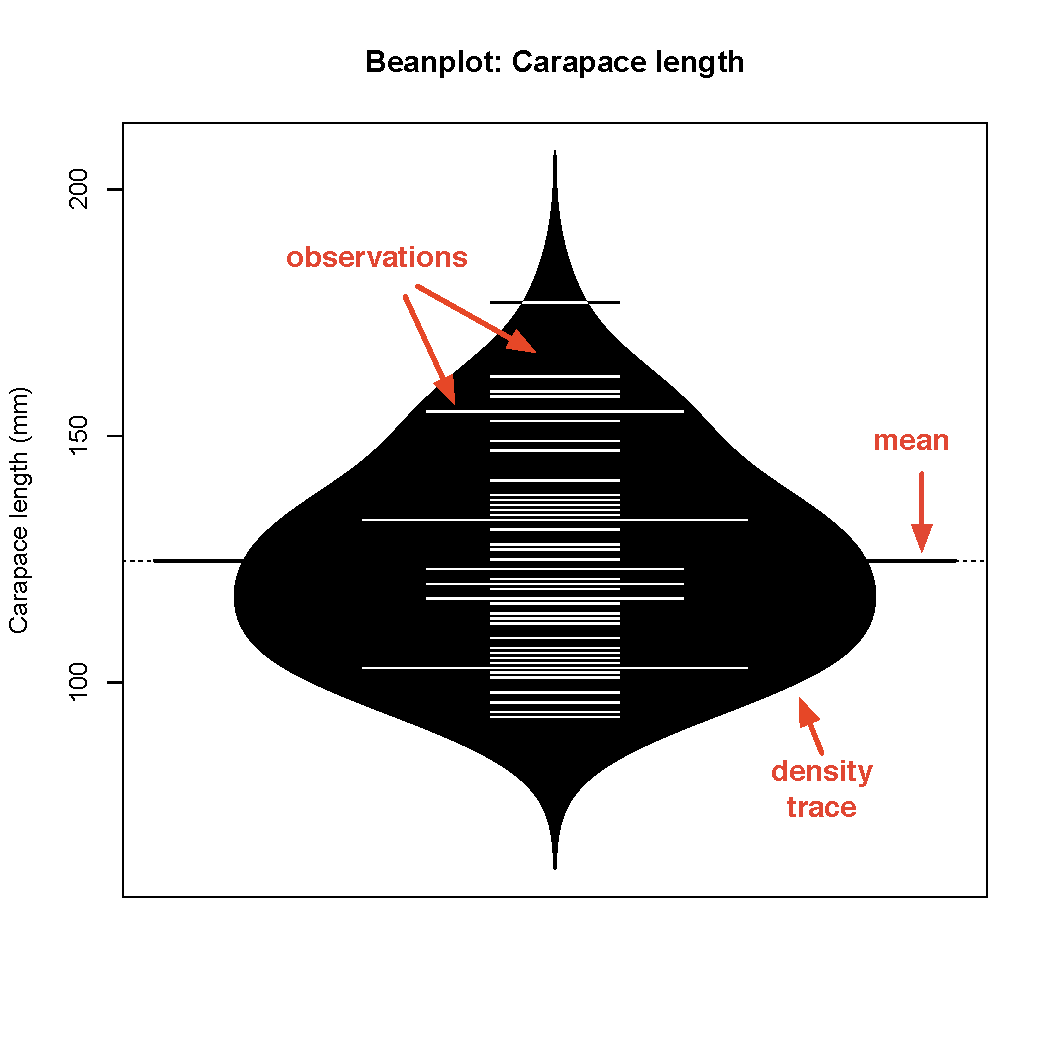
\includegraphics[width=0.5\columnwidth]{./figures/hands-on2/beanplot-labeled.pdf}
\caption{Beanplots combine features of density and box plots.}
\end{figure}

The \lstinline!beanplot! package is not installed by default. To
download it and install it use the R package installer under the
\lstinline!Packages & Data! menu. If this
is the first time you use the package installer you'll have to choose a
CRAN repository from which to download package info (I recommend you
pick one in the US). Once you've done so you can search for `beanplot'
from the Package Installer window. You should also check the 'install
dependencies' check box.

Once the beanplot package has been installed check out the examples to
see some of the capabilities:

\begin{R}
> library(beanplot)
> example(beanplot)
\end{R}

Note the use of the \lstinline!library()! function to make the functions
in the \lstinline!beanplot! library available for use. Here's some
examples of using the \lstinline!beanplot! function with the turtle data
set:

\begin{R}
> beanplot(turtles$length) # note the message about log='y'
> beanplot(turtles$length, log='') # DON'T do the automatic log transform
> beanplot(turtles$length, log='', col=c('white','blue','blue','red'))
\end{R}
In the final version we specified colors for the parts of the beanplot.
See the explanation of the \lstinline!col! argument int he beanplot
function for details.

We can also compare the carapace length variable for male and female
turtles.

\begin{R}
> beanplot(length ~ sex, data = turtles, col=list(c('red'),c('black')),
names = c('females','males'),xlab='Sex', ylab='Caparace length (mm)')
\end{R}
Note the use of the formula notation to compare the carapace length
variable for males and females. There is also a asymmetrical version of
the beanplot which can be used to more directly compare distributions
between two groups. We explore this below. Note too the use of the list
argument to \lstinline!col!, and the use of vectors within the list to
specify the colors for female and male beanplots.

We can also create a beanplot with multiple variables in the same plot
if the variables are measured on the same scale.

\begin{R}
> beanplot(turtles$length, turtles$width, turtles$height, log='',
names=c('length','width','height'), ylab='carapace dimensions (mm)')
\end{R}



\subsection{Demo Plots in R}

To get a sense of some of the graphical power of R try the
\lstinline!demo()! function:
%
\begin{R}
> demo(graphics)
\end{R}


%!TEX root = ./hands-on1.tex

\subsection{Sweave for R}

Sweave documents weave together documentation/discussion and code into a
single document. The pieces of code and documentation are referred to as
`chunks'. R comes with a set of tools that allow you to extract just the
code, or to turn the entire document into a nicely formatted report.

Here's a simple Sweave document to get you started:
%
\begin{noindentcodeblock}[tex]
\documentclass{article}
\begin{document}

This is a very simple Sweave file. It includes only a single code chunk.

<<>>=
z <- rnorm(30, mean=0, sd=1)
summary(z)
@

That code chunk generated a random sample of 30 observations drawn from a normal distribution with mean zero and standard deviation one.

\end{document}  
\end{noindentcodeblock}
%
Type those lines into a text editor and save the document with the name
|sweave1.Rnw|.

Let's break down the various pieces of the document. The first two lines
and the last line represent LaTeX~commands.

\begin{code}{tex}
\documentclass{article}
\begin{document}
    ....
\end{document}
\end{code}
For simple Sweave documents that's all the LaTeX you need to learn.
However, learning a little bit more about the document preparation
system gives you the option of producing very nicely formatted output as
we'll see in a little bit.

The R code is preceeded by the text |<<>>=|. This tells Sweave
that you're starting a code chunk. The |@| symbol after the
code chunk tells Sweave that you're going back to writing documentation
chunks.

If you already have a working installation of LaTeX on your computer you
can now compile this into a nicely formatted document from the R
interpretter. Change the R working directory so that it's in the same
directory where you saved the |sweave1.Rnw| file. The execute
the following commands:
%
\begin{R}
> library(tools)  # makes the texi2dvi function available
> Sweave('sweave1.Rnw') # compiles our Sweave document into 'sweave1.tex'
> texi2dvi("sweave1.tex", pdf = TRUE)
\end{R}
%
These commands will produce two new documents -- |sweave1.tex|
and a PDF document, |sweave1.pdf|. You can open the
|sweave1.tex| file in any text editor and you'll see that it's
just a slightly modified version of the |sweave1.Rnw| file you
created. The PDF file contains the nicely formatted report.

If you got an error message the most likely reason is that R can't find
the path to your LaTeX executable. To check this try:
%
\begin{R}
> texi2dvi('sweave1.tex', pdf=TRUE, quiet=FALSE)
\end{R}
%
If that's the case, you can fix that by typing the following into the R
command line (on OS X):
%
\begin{R}
> Sys.setenv("PATH" = paste(Sys.getenv("PATH"),"/usr/texbin",sep=":"))  
\end{R}
%
Then try executing the |texi2dvi| command again. If that
solved your problem you can make this permanent by adding that line to
your |.Rprofile| (located in |/Users/yourname| on \OSX; if the
file doesn't already exist go ahead and create it). If that doesn't work
please see me for troubleshooting help.

\subsubsection{RStudio makes Sweaving easy!}

RStudio hides some of the complexity of Sweaving documents. Simply
create or open your Sweave document (use the .Rnw extension) in RStudio
and then hit the |Compile PDF| button. If your LaTeX setup is
working, and the document and code are valid, Rstudio will compile
everything behind the scenes and pop up a nice PDF.

\subsubsection{A fancier Sweave document}

Let's get a little bit fancier and show how we can create graphics and
use some LaTeX formatting features to produce a nicer document.

\begin{codeblock}[tex]
\documentclass[letterpaper]{article}
\usepackage[margin=0.75in]{geometry}

\title{My Second Sweave Report}
\author{John Q. Public}

\begin{document}
\maketitle
This is a still a simple Sweave file. However, now it includes several code chunks and several \LaTeX\ specific commands.

\section{Sampling from the random normal distribution}

<<>>=
z <- rnorm(30, mean=0, sd=1)
summary(z)
@

That code chunk generated a random sample of 30 observations drawn from a normal distribution with mean zero ($\mu = 0$) and standard deviation one ($\sigma = 1$).

\section{Generating figures}

We can also automatically imbed graphics in our report. For example, the following will generate a histogram.

% this tells Sweave to set the graphics 
% to be half the width of the text
\setkeys{Gin}{width=0.5\textwidth} 
<<fig=TRUE>>=
hist(z)
@

\end{document}    
\end{codeblock}
%
Notice how we put an argument, |fig=TRUE| within the second
code chunk delimiter. This will tell Sweave to automatically imbed a
figure with the histogram graphic we created into our report. Save this
as |sweave2.Rnw| and repeat the above steps to compile it into
a PDF report.

For a full overview of Sweave's capabilities see the documentation for
Sweave availabe at
\url{http://www.stat.uni-muenchen.de/~leisch/Sweave/}.

\subsection{Pweave for literate programming in Python}

Pweave uses almost exactly the same syntax as Sweave to delimit code and
document chunks. Here's a simple Pweave document.

\begin{codeblock}[tex]
\documentclass[letterpaper]{article}
\usepackage[margin=0.75in]{geometry}
\usepackage{graphicx} % unlike Sweave, Pweave doesn't
                      % pull this in automatically

\title{My First Pweave Report}
\author{John Q. Public}

\begin{document}
\maketitle
This is a still a simple Pweave file. As in our Sweave example,
there are several code chunks and we've included a figure.

\section{Sampling from the random normal distribution}

<<>>=
from numpy import random
z = random.normal(loc=0, scale=1, size=30)
@

That code chunk generated a random sample of 30 
observations drawn from a normal distribution with mean 
zero ($\mu = 0$) and standard deviation one ($\sigma = 1$).

\section{Generating figures}

We can also automatically imbed graphics in our 
report. For example, the following will generate 
a histogram.

% this tells Sweave to set the graphics 
% to be half the width of the text
\setkeys{Gin}{width=0.5\textwidth} 
<<fig=True>>=
import pylab
pylab.hist(z)
@

\end{document}
\end{codeblock}
%
Note that the second code chunk, we wrote |fig=True| in the
Pweave document, whereas we wrote |fig=TRUE| for the Sweave
document. This minor difference reflects the different syntax for
boolean values in R and Python.

Save that code in a text file called |pweave1.Pnw| and from
the bash shell (\emph{not} in the Python interpretter) type the
following command:
%
\begin{bash}
Pweave -f "tex" pweave1.Pnw
\end{bash}
%
The option |-f "tex"| tells Pweave to output a file (Note:
from the Windows command prompt you must use double quotes around
``tex'', on Unix-based systems either single our double quotes work
fine). Assuming you got no error messages, you can then compile this to
PDF using the following command:
%
\begin{bash}
pdflatex pweave1.tex
\end{bash}



\chapter{Bivariate Data}

%!TEX root = ./workbook-2011.tex

\section{Vector Operations in R}

As you saw last week R vectors support basic arithmetic operations that
correspond to the same operations on geometric vectors. For example:
%
\begin{R}
> x <- 1:15
> y <- 10:24
> x
 [1]  1  2  3  4  5  6  7  8  9 10 11 12 13 14 15
> y
 [1] 10 11 12 13 14 15 16 17 18 19 20 21 22 23 24

> x + y             # vector addition
 [1] 11 13 15 17 19 21 23 25 27 29 31 33 35 37 39
> x - y             # vector subtraction
 [1] -9 -9 -9 -9 -9 -9 -9 -9 -9 -9 -9 -9 -9 -9 -9
> x * 3             # multiplication by a scalar
 [1]  3  6  9 12 15 18 21 24 27 30 33 36 39 42 45
\end{R}
%
R also has an operator for the dot product, denoted \lstinline!%*%!.
This operator also designates matrix multiplication, which we will
discuss next week. By default this operator returns an object of the R
matrix class. If you want a scalar (or the R equivalent of a scalar,
i.e.~a vector of length 1) you need to use the \lstinline!drop()!
function.

\begin{R}
> z <- x %*% x
> class(z)      # note use of class() function
[1] "matrix"
> z
     [,1]
[1,] 1240
> drop(z)
[1] 1240
\end{R}

In lecture we saw that many useful geometric properties of vectors could be expressed in the form of dot products. Let's start with some two-dimensional vectors where the geometry is  easy to visualize:

\begin{R}
> a <- c(1, 0) # the point (1,0)
> b <- c(0, 1) # the point (0,1)
\end{R}
%
Now let's draw our vectors:
%
\begin{R}
# create empty plot w/specified x- and y- limits
# the 'asp=1' argument maintains the scaling of the x- and y-axes
# so that units are equivalent for both axes (i.e. squares remain squares)
> plot(c(-2,2),c(-1,2),type='n', asp=1)

# draw an arrow from origin (0,0) to x,y coordinates of vector "a"
# the length argument changes the size of the arrowhead
# use the R help to read more about the arrows function
> arrows(0, 0, a[1], a[2], length=0.1)

# and now for the vector "b"
> arrows(0, 0, b[1], b[2], length=0.1)
\end{R}
%
You should now have a figure that looks like the one below:
\begin{figure}[htbp]
\centering
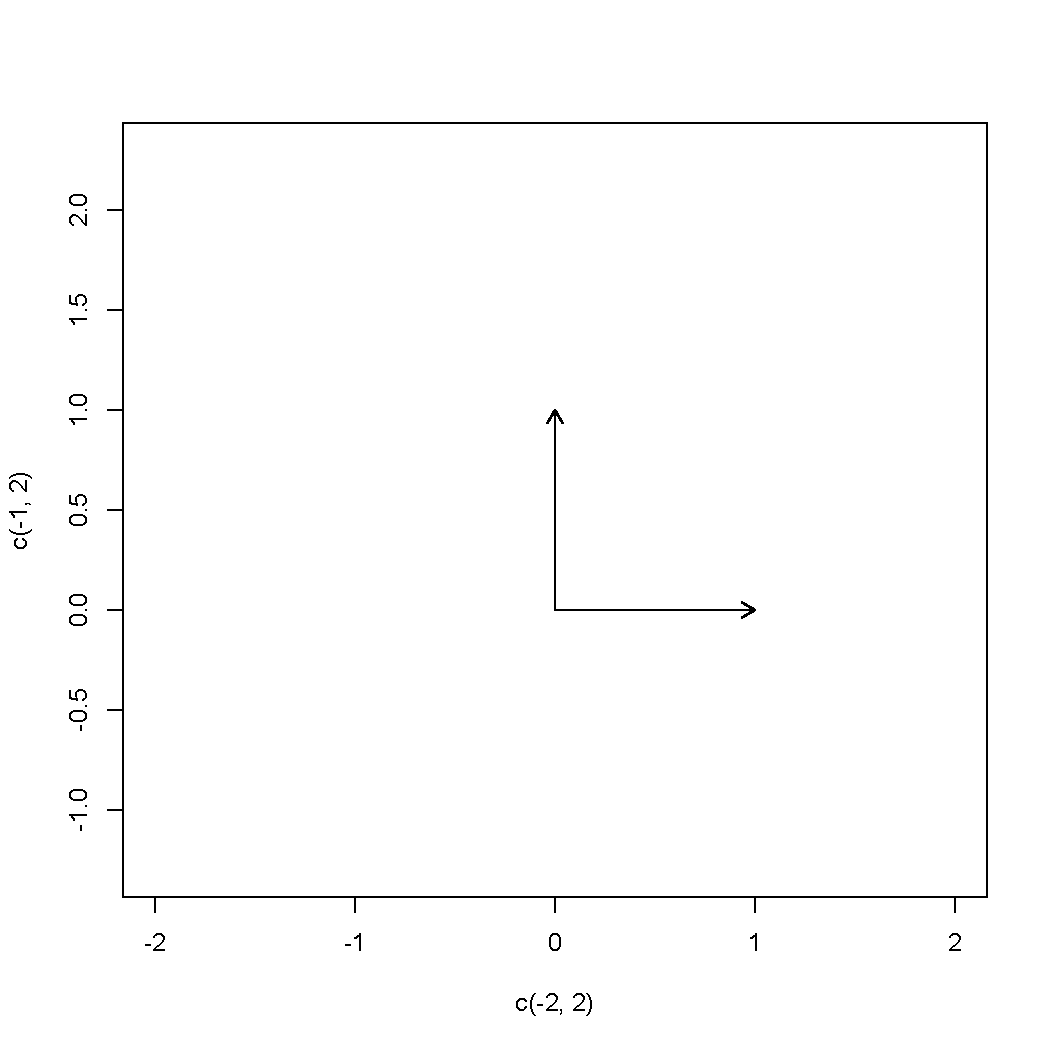
\includegraphics[width=0.33\columnwidth]{./figures/hands-on2/rightangle.pdf}
\caption{A simple vector figure.}
\end{figure}
%
Let's see what the dot product can tell us about these vectors. First recall that we can calculate the length of a vector as the square-root of the dot product of the vector with itself ($\vert\vec{a}\vert^2  =  \vec{a} \cdot \vec{a}$)
\begin{R}
> len.a <- drop(sqrt(a %*% a))
> len.a
[1] 1
> len.b <- drop(sqrt(b %*% b))
\end{R}
%
How about the angle between $a$ and $b$?
\begin{R}
> dot.ab <- a %*% b
> dot.ab
     [,1]
[1,]    0
> cos.ab <- (a %*% b)/(len.a * len.b)
> cos.ab
     [,1]
[1,]    0
\end{R}
A key point to remember dot product of two vectors is zero if, and only if, they are orthogonal to each other (regardless of their dimension).




%!TEX root = ./workbook-2011.tex

\section{Writing Functions in R}

So far we've been mostly using R's built in functions. However the power of a
true programming language is the ability to write your own functions.

The general form of an R function is as follows:

\begin{R}
funcname <- function(arg1, arg2) {
 # one or more expressions
 # last expression is the object returned
 # or you can explicitly return an object
}
\end{R}
To make this concrete, here's an example where we define a function in
the interpreter and then put it to use:
%
\begin{R}
> myfunc <- function(x,y){
+ # don't type the '+' symbols, these show continuation lines
+   x^2 + y^2
+ }

> a <- 1:5
> b <- 6:10
> a
[1] 1 2 3 4 5
> b
[1]  6  7  8  9 10
> myfunc(a,b)
[1]  37  53  73  97 125
> myfunc
function(x,y){
  x^2 + y^2
}
\end{R}
%
If you type a function name without parentheses R shows you the
function's definition. This works for built-in functions as well
(thought sometimes these functions are defined in C code in which case R
will tell you that the function is a `.Primitive').

\subsection{Putting R functions in Scripts}

When you define a function at the interactive prompt and then close the
interpreter your function definition will be lost. The simple way around
this is to define your R functions in a script that you can than access
at any time.

Choose \lstinline!File > New Script! (or \lstinline!File > New Document! in OS
X) in the R GUI . This
will bring up a blank editor window. Enter your function into the editor
and save the source file in your R working directory with a name like
\lstinline!vecgeom.R!.

\begin{R}
# functions defined in vecgeom.R

veclength <- function(x) {
  # Given a numeric vector, returns length of that vector
  sqrt(drop(x %*% x))
}

unitvector <- function(x) {
  # Return a unit vector in the same direction as x
  x/veclength(x)
}

vec.cos <- function(x,y) {
  # Calculate the cos of the angle between vectors x and y
  len.x <- veclength(x)
  len.y <- veclength(y)
  return( (x %*% y)/(len.x * len.y) )
}

\end{R}
There are two functions defined above, one of which calls the other.
Both take single vector arguments. At this point there is no error
checking to insure that the argument is reasonable but R's built in
error handling will do just fine for now.

Once your functions are in a script file you can make them accesible by
using the \lstinline!source()! function (See also the
\lstinline!File > Source R code...! menu item in the R GUI):
%
\begin{R}
> source("vecgeom.R")
> x <- c(1,0.4)
> veclength(x)
[1] 1.077033
> ux <- unitvector(x)
> ux
[1] 0.9284767 0.3713907
> veclength(ux)
[1] 1
\end{R}

Let's also add the following function to |vecgeom.R| to aid in visualizaing 2D vectors:
%
\begin{R}
draw.vectors <- function(a, b, colors=c('red', 'blue'), clear.plot=TRUE){

    # figure out the limits such that the origin and the vector
    # end points are all included in the plot
    xhi <- max(0, a[1], b[1])
    xlo <- min(0, a[1], b[1])
    yhi <- max(0, a[2], b[2])
    ylo <- min(0, a[2], b[2])

    xlims <- c(xlo, xhi)*1.10 # give a little breathing space around vectors
    ylims <- c(ylo, yhi)*1.10

    if (clear.plot){
        plot(xlims, ylims, type='n', asp=1, xlab="x-coord", ylab="y-coord")
    }
    arrows(0, 0, a[1], a[2], length=0.1, col=colors[1])
    arrows(0, 0, b[1], b[2], length=0.1, col=colors[2])
}
\end{R}
%
You can use this new function as follows:
\begin{R}
# you need to source the file everytime you change it
> source("/Users/pmagwene/Downloads/vecgeom.R")
> x <- c(1,0.4)
> y <- c(0.2, 0.8)
> draw.vectors(x,y)  # draw the original vectors
\end{R}
%
The resulting figure should resemble the one below.
%
\begin{figure}[htbp]
\centering
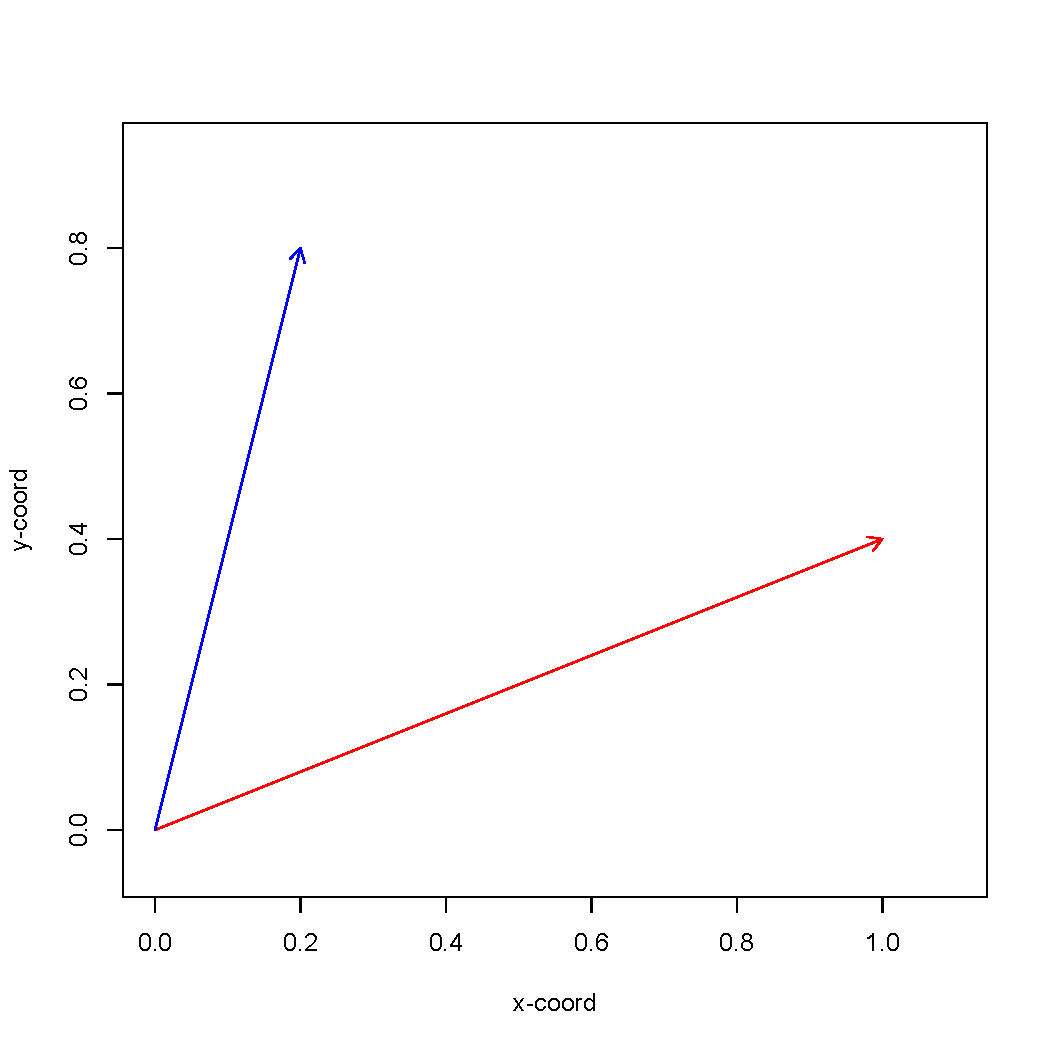
\includegraphics[width=0.33\columnwidth]{./figures/hands-on2/vecfig2.pdf}
\caption{Another vector figure.}
\end{figure}

Notice that we included a |clear.plot| argument in our |draw.vectors| function. I included this so we could add additional vectors to our plot, without overwriting the old vectors, as demonstrated below:
\begin{R}
# draw the unit vectors that point in the same directors as the original vectors
> ux <- unitvector(x)
> uy <- unitvector(y)
> draw.vectors(ux, uy, colors=c('black', 'green'), clear.plot=F)
\end{R}

\begin{assignment}
Write a function in R that takes two vectors, $\vec{x}$ and $\vec{y}$, and returns a list containing the projection of $\vec{y}$ on $\vec{x}$ and the component of $\vec{y}$ in $\vec{x}$:

\lstDeleteShortInline|

\[P_{\vec{x}}(\vec{y}) = \left(\frac{\vec{x} \cdot \vec{y}}{|\vec{x}|}\right) \frac{\vec{x}}{|\vec{x}|}\]
and
\[C_{\vec{x}}(\vec{y}) = \frac{\vec{x} \cdot \vec{y}}{|\vec{x}|}\]

\lstMakeShortInline|

\end{assignment}



%%!TEX root = ./workbook-2011.tex

\section{Basic statistical functions in R}

\subsection{Dealing with Data Subsets in R}

Manipulating or analyzing subsets of data is one of the most common
tasks in R. The \lstinline!subset()! function comes in handy for such
operations. Consider the data set \lstinline!turtles.txt!:
%
\begin{R}
> turtles <- read.table('turtles.txt', header=T)
> turtles
   sex length width height
1    f     98    81     38
2    f    103    84     38
3    f    103    86     42
  # output truncated
> names(turtles)
[1] "sex"    "length" "width"  "height"
> # Now we'll apply the subset() function
> turt.sub <- subset(turtles, select = -sex)
> names(turt.sub)
[1] "length" "width"  "height"
> turt.sub
   length width height
1      98    81     38
2     103    84     38
3     103    86     42
  # output truncated
\end{R}
%
In the example above we create a subset of the original data set by
excluding the variable indicating the sex of each individual using the
argument \lstinline!select = -sex!. We can also explicit include only
certain variables, like this:
%
\begin{R}
> turt.sub2 <- subset(turtles, select=c(height,width))
> turt.sub2
   height width
1      38    81
2      38    84
3      42    86
  # output truncated    
\end{R}
%
\lstinline!subset()! allows you to do more than just select variables to
include. You can use the second positional argument to specify matching
criteria. For example:
%
\begin{R}
# gives only female turtles, all variables except sex
> female.turts <- subset(turtles, sex == "f", select = -sex)
> dim(female.turts)
[1] 24  3
# same for male turtles
> male.turts <- subset(turtles, sex == "m", select = -sex)
> dim(male.turts)
[1] 24  3
# gives only females with length > 125, all variables
> big.females <- subset(turtles, sex == "f" & length > 125)    
\end{R}

The \lstinline!subset! function is especially useful when combined with
the function \lstinline!sapply()! which allows you to apply a function
of interest to each variable. For example:
%
\begin{R}
> min(turtles)
Error in Summary.data.frame(..., na.rm = na.rm) : 
        only defined on a data frame with all numeric or complex variables
> min(turt.sub)  # unexpected result
[1] 35
> sapply(turt.sub, min) # here's what we were shooting for
length  width height 
    93     74     35
> sapply(female.turts, min) # for females
length  width height 
    98     81     38 
> sapply(male.turts, min) # for males
length  width height 
    93     74     35      
\end{R}
%
Notice how the \lstinline!min()! function chokes on the complete data
set because the function is not defined for factor variables. In the
second example \lstinline!min(turt.sub)! returns a valid result, but
also not exactly what we wanted. In this case it looked for the minimum
value across all the objects passed to it. In the third case we use the
\lstinline!sapply()! function and get the minimum on a
variable-by-variable basis. Please take a moment to look at the
documentation for the \lstinline!sapply()! function and cook up some
examples of your own.

\paragraph{Anderson's (Fisher's) iris data set}

Anderson's (or Fisher's) iris data set consists of four morphometric
measurements for specimens from three different iris species. Use the R
help to read about the iris data set (\lstinline!?iris!). We'll be using
this data set repeatedly in future weeks so familiarize yourself with
it.

\smallskip
\begin{assignment}
Calculate a summary table as well as correlation
and covariance matrices for each of the species in the iris data set.
Use \lstinline!help.search()! and \lstinline!apropos()! to lookup any
necessary function names.
\end{assignment}


\subsection{Exploring Univariate Distributions in R}

\subsubsection{Histograms}

One of the most common ways to examine a the distribution of
observations for a single variable is to use a histogram. The
\lstinline!hist()! function creates simple histograms in R.

\begin{R}
> hist(turtles$length) # create histogram with fxn defaults
> ?hist # check out the documentation on hist
\end{R}
Note that by default the \lstinline!hist()! function plots the
frequencies in each bin. If you want the probability densities instead
set the argument \lstinline!freq=FALSE!.
%
\begin{R}
> hist(turtles$length,freq=F) # y-axis gives probability density
\end{R}
Here's some other ways to fine tune a histogram in R.

\begin{R}
> hist(turtles$length, breaks=12) # use 12 bins
> mybreaks = seq(85,185,8)
> hist(turtles$length, breaks=mybreaks) # specify bin boundaries   
> hist(turtles$length, breaks=mybreaks, col='red') # fill the bins with red  
\end{R}

\subsubsection{Density Plots}

One of the problems with histograms is that they can be very sensitive
to the size of the bins and the break points used. This is due to the
discretization inherent in a histogram. A `density plot' or `density
trace' is a continuous estimate of a probability distribution from a set
of observations. Because it is continuous it doesn't suffer from the
same sensitivity to bin sizes and break points. One way to think about a
density plot is as the histogram you'd get if you averaged many
individual histograms each with slightly different breakpoints.
%
\begin{R}
> d <- density(turtles$length)
> plot(d)    
\end{R}
%
A density plot isn't entirely parameter free -- the parameter you should
be most aware of is the `smoothing bandwidth'.

\begin{R}
> d <- density(turtles$length) # let R pick the bandwidth
> plot(d,ylim=c(0,0.020)) # gives ourselves some extra headroom on y-axis
> d2 <- density(turtles$length, bw=5) # specify bandwidth
> lines(d2, col='red') # use lines to draw over previous plot
\end{R}
The bandwidth determines the standard deviation of the `kernel' that is
used to calculate the density plot. There are a number of different
types of kernels you can use; a Gaussian kernel is the R default and is
the most common choice. See the documentation for more info.

The \lstinline!lattice! package is an R library that makes it easier to
create graphics that show conditional distributions. Here's how to
create a simple density plot using the \lstinline!lattice! package.

\begin{R}
> library(lattice)
> densityplot(turtles$length) # densityplot defined in lattice
\end{R}
Notice how by default the \lstinline!lattice! package also drew points
representing the observations along the x-axis. These points have been
`jittered' meaning they've been randomly shifted by a small amount so
that overlapping points don't completely hide each other. We could have
produced a similar plot, without the lattice package, as so:

\begin{R}
> d <- density(turtles$length)
> plot(d)
> nobs <- length(turtles$length)
> points(jitter(turtles$length), rep(0,nobs)) 
\end{R}
Notice that in our version we only jittered the points along the x-axis.
You can also combine a histogram and density trace, like so:

\begin{R}
> hist(turtles$length, 10, xlab='Carapace Length (mm)',freq=F)
> d <- density(turtles$length)
> lines(d, col='red', lwd=2) # red lines, with pixel width 2    
\end{R}
Notice the use of the \lstinline!freq=F! argument to scale the histogram
bars in terms of probability density.

Finally, let's some of the features of \lstinline!lattice! to produce
density plots for the `length' variable of the turtle data set,
conditional on sex of the specimen.

\begin{R}
> densityplot(~length | sex, data = turtles)    
\end{R}
There are a number of new concepts here. The first is that we used what
is called a `formula' to specify what to plot. In this case the formula
can be read as `length conditional on sex'. We'll be using formulas in
several other contexts and we discuss them at greater length below. The
\lstinline!data! argument allows us to specify a data frame or list so
that we don't always have to write arguments like
\lstinline!turtles$length! or \lstinline!turtles$sex! which can get a
bit tedious.

\subsubsection{Box Plots}

Another common tool for depicting a univariate distribution is a `box
plot' (sometimes called a box-and-whisker plot). A standard box plot
depicts five useful features of a set of observations: the median
(center most line), the upper and lower quartiles (top and bottom of the
box), and the minimum and maximum observations (ends of the whiskers).

\begin{figure}[htbp]
\centering
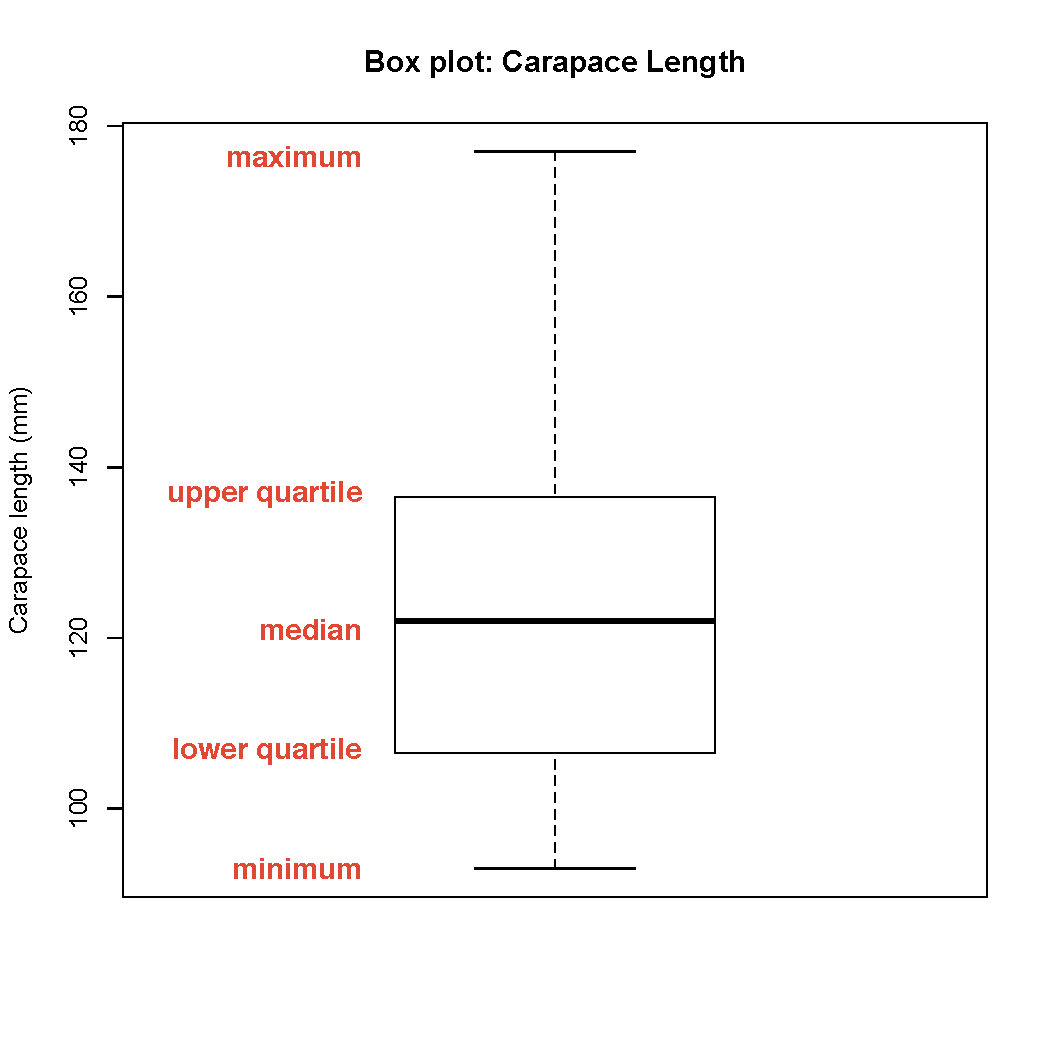
\includegraphics[width=0.5\columnwidth]{./figures/hands-on2/boxplot-labeled.pdf}
\caption{A box plot represents a five number summary of a set of
observations.}
\end{figure}

There are many variants on box plots, particularly with respect to the
`whiskers'. It's always a good idea to be explicit about what a box plot
you've created depicts.

Here's how to create box plots using the standard R functions as well as
the lattice package:

\begin{R}
> boxplot(turtles$length)
> boxplot(turtles$length, col='darkred', horizontal=T) # horizontal version 
> title(main = 'Box plot: Carapace Length', ylab = 'Carapace length (mm)')
> bwplot(~length,data=turtles) # using the bwplot function from lattice
\end{R}
Note how we used the \lstinline!title()! function to change the axis
labels and add a plot title.

\paragraph{Historical note}

-- The box plot is one of many inventions of the statistician John W.
Tukey. Tukey made many contributions to the field of statistics and
computer science, particularly in the areas of graphical representations
of data and exploratory data analysis.

\subsubsection{Bean Plots}

My personal favorite way to depict univariate distributions is called a
`beanplot'. Beanplots combine features of density plots and boxplots and
provide information rich graphical summaries of single variables. The
standard features in a beanplot include the individual observations
(depicted as lines), the density trace estimated from the observations,
the mean of the observations, and in the case of multiple beanplots an
overall mean.

\begin{figure}[htbp]
\centering
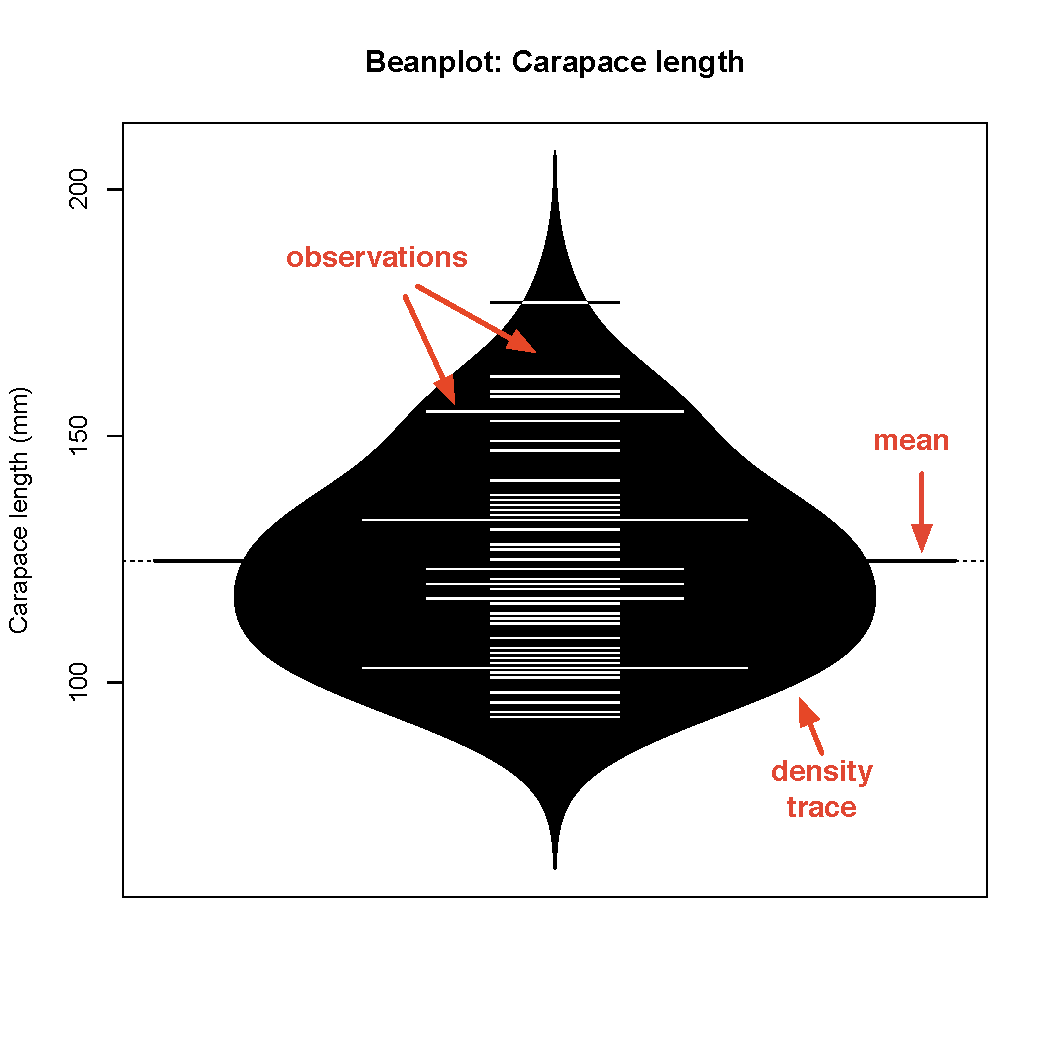
\includegraphics[width=0.5\columnwidth]{./figures/hands-on2/beanplot-labeled.pdf}
\caption{Beanplots combine features of density and box plots.}
\end{figure}

The \lstinline!beanplot! package is not installed by default. To
download it and install it use the R package installer under the
\lstinline!Packages & Data! menu (standard R GUI) or in
\lstinline!Tools > Install Packages...! in RStudio (see also the
\lstinline!Packages! tab in the lower-right window in RStudio). If this
is the first time you use the package installer you'll have to choose a
CRAN repository from which to download package info (I recommend you
pick one in the US). Once you've done so you can search for `beanplot'
from the Package Installer window. You should also check the 'install
dependencies' check box.

Once the beanplot package has been installed check out the examples to
see some of the capabilities:

\begin{R}
> library(beanplot) 
> example(beanplot)    
\end{R}
If you ran the examples in RStudio, use the \lstinline!Clear All! option
in the \lstinline!Plots! tab after running the examples in order to
reset parameters that the examples changed.

Note the use of the \lstinline!library()! function to make the functions
in the \lstinline!beanplot! library available for use. Here's some
examples of using the \lstinline!beanplot! function with the turtle data
set:

\begin{R}
> beanplot(turtles$length) # note the message about log='y'
> beanplot(turtles$length, log='') # DON'T do the automatic log transform
> beanplot(turtles$length, log='', col=c('white','blue','blue','red'))
\end{R}
In the final version we specified colors for the parts of the beanplot.
See the explanation of the \lstinline!col! argument int he beanplot
function for details.

We can also compare the carapace length variable for male and female
turtles.

\begin{R}
> beanplot(length ~ sex, data = turtles, col=list(c('red'),c('black')),
names = c('females','males'),xlab='Sex', ylab='Caparace length (mm)')
\end{R}
Note the use of the formula notation to compare the carapace length
variable for males and females. There is also a asymmetrical version of
the beanplot which can be used to more directly compare distributions
between two groups. We explore this below. Note too the use of the list
argument to \lstinline!col!, and the use of vectors within the list to
specify the colors for female and male beanplots.

We can also create a beanplot with multiple variables in the same plot
if the variables are measured on the same scale.

\begin{R}
> beanplot(turtles$length, turtles$width, turtles$height, log='',
names=c('length','width','height'), ylab='carapace dimensions (mm)') 
\end{R}


\subsection{Simple t-tests in R}

Student's t-tests can be carried out in R using the function
\lstinline!t.test()!. The \lstinline!t.test()! function can perform one
and two-sample t-tests (i.e.~comparing a sample of interest against a
hypothesized mean, or comparing the means of two samples). The
\lstinline!t.test()! function also supports a `formula' interface for
two-sample t-tests similar to the \lstinline!lm(!) function.

\begin{R}
> t.test(width ~ sex, data=turtles)

        Welch Two Sample t-test

data:  width by sex 
t = 4.7015, df = 35.355, p-value = 3.862e-05
alternative hypothesis: true difference in means is not equal to 0 
95 percent confidence interval:
  8.122699 20.460634 
sample estimates:
mean in group f mean in group m 
      102.58333        88.29167 
\end{R}
The asymmetric version of the boxplot is very useful for comparing
distributions of the same variable between two groups. To generate such
plots use the argument \lstinline!side='both'! as an argument to
\lstinline!beanplot!.

\begin{R}
> beanplot(width ~ sex, data = turtles, side='both', col=list(c('red'),c('black')))  
\end{R}
As you can see this splits the beanplot in half for each group and puts
them back to back to facilitate comparison. The difference in the mean
of the two groups is visually obvious from the beanplot.

\begin{assignment}
\begin{enumerate}[a)]
\item
  Prepare beanplots showing samples grouped by \lstinline!Species! for
  each of the quantitative variables in the iris data set. Label the x-
  and y-axes of your boxplots and give each plot a title. \textbf{Tip}: since there are three species, you can't use the \lstinline!side='both'! argument, and you'll need to extend the \lstinline!col=list! argument to add a third color.

\item Carry out two-sample t-tests contrasting \lstinline!versicolor! and
  \lstinline!virginica! for each of the four morphometric variables in
  the iris data set. \textbf{Tip}: use the \lstinline!subset()! function to create a subset of the iris data containing just these two species.

\item Write a brief paragraph interpreting the results of the t-tests you
  conducted.
\end{enumerate}
\end{assignment}

\subsection{Exploring Bivariate Distributions in R}

\subsubsection{Scatterplots}

When dealing with pairs of continuous variables a scatter plot is the
obvious choice. The standard \lstinline!plot! function can be used:

\begin{R}
> plot(turtles$length, turtles$width)
> plot(turtles$length ~ turtles$width)    
\end{R}
Did you notice what is different between the two versions above? You can
also use the \lstinline!data! argument with plot, like so:

\begin{R}
> plot(length ~ width, data=turtles)
\end{R}
The \lstinline!xyplot()! function from the \lstinline!lattice! package
does pretty much the same thing:
%
\begin{R}
> xyplot(length ~ width, data = turtles)
\end{R}


\subsubsection{Regression in R}

R has very flexible built in functions for fitting linear models.
Bivariate regression is the simplest case of a linear model.

\begin{R}
> turtles <- read.table('turtles.txt',header=T)
> names(turtles)
[1] "sex"    "length" "width"  "height"
> regr <- lm(turtles$width ~ turtles$length)
> class(regr)
[1] "lm"
> names(regr)
 [1] "coefficients"  "residuals"     "effects"       "rank"          "fitted.values"
 [6] "assign"        "qr"            "df.residual"   "xlevels"       "call"         
[11] "terms"         "model"   
> summary(regr)

Call:
lm(formula = turtles$width ~ turtles$length)

Residuals:
     Min       1Q   Median       3Q      Max 
-5.57976 -1.66578 -0.04471  1.73752  5.97104 

Coefficients:
               Estimate Std. Error t value Pr(>|t|)    
(Intercept)     19.9434     2.3877   8.353 8.99e-11 ***
turtles$length   0.6055     0.0189  32.033  < 2e-16 ***
---
Signif. codes:  0 '***' 0.001 '**' 0.01 '*' 0.05 '.' 0.1 ' ' 1 

Residual standard error: 2.654 on 46 degrees of freedom
Multiple R-Squared: 0.9571,     Adjusted R-squared: 0.9562 
F-statistic:  1026 on 1 and 46 DF,  p-value: < 2.2e-16 

> plot(turtles$width ~ turtles$length)  # scatter plot with turtles$length on x axis
> abline(regr)  # plot the regression line
\end{R}
Note the use of the function \lstinline!abline()! to plot the regression
line. Calling \lstinline!plot()! with an object of class \lstinline!lm!
shows a series of diagnostic plots. Try this.

\begin{assignment}
Write your own regression function (i.e.~your
code shouldn't refer to the built in regression functions) for mean
centered vectors in R. The function will take as it's input two vectors,
$\vec{x}$ and $\vec{y}$. The function should return:

\begin{enumerate}[1.]
\item
  a list containing the mean-centered versions of these vectors
\item
  the regression coefficient $b$ in the mean centered regression
  equation $\vec{\widehat{y}} = b\vec{x}$
\item
  the coefficient of determination, $R^2$
\end{enumerate}
Demonstrate your regression function by using it to carry out
regressions of Sepal.Length on Sepal.Width separately for the `setosa'
and `virginica' specimens from the iris data set (again,
\lstinline!subset()! is your friend). Include plots in which you use the
\lstinline!plot()! and \lstinline!abline()! functions to illustrate your
calculated regression line.

\end{assignment}




\chapter{Matrices and matrix operations in R}


\section{Matrices in R}

In R matrices are two-dimensional collections of elements all of which
have the same mode or type. This is different than a data frame in which
the columns of the frame can hold elements of different type (but all of
the same length), or from a list which can hold objects of arbitrary
type and length. Matrices are more efficient for carrying out most
numerical operations, so if you're working with a very large data set
that is amenable to representation by a matrix you should consider using
this data structure.

\subsection{Creating matrices in R}

There are a number of different ways to create matrices in R. For
creating small matrices at the command line you can use the
\lstinline!matrix()! function.

\begin{R}
> X <- matrix(1:5)
> X
      [,1]
 [1,]    1
 [2,]    2
 [3,]    3
 [4,]    4
 [5,]    5
> X <- matrix(1:12, nrow=4)
> X
     [,1] [,2] [,3]
[1,]    1    5    9
[2,]    2    6   10
[3,]    3    7   11
[4,]    4    8   12
> dim(X) # give the shape of the matrix 
[1] 4 3
\end{R}
\lstinline!matrix()! takes a data vector as input and the shape of the
matrix to be created is specified by using the \lstinline!nrow! and
\lstinline!ncol! arguments (if the number of elements in the input data
vector is less than |nrows| $\times$ |ncols| the
elements will be 'recycled' as discussed in previous lectures). Without
any shape arguments the \lstinline!matrix()! function will create a
column vector as shown above. By default the \lstinline!matrix()!
function fills in the matrix in a column-wise fashion. To fill in the
matrix in a row-wise fashion use the argument \lstinline!byrow=T!.

If you have a pre-existing data set in a list or data frame you can use
the \lstinline!as.matrix()! function to convert it to a matrix.

\begin{R}
> turtles <- read.table('turtles.txt', header=T)
> tmtx <- as.matrix(turtles) 
> tmtx   # note how the elements were all converted to character 
   sex length width height
1  "f" " 98"  " 81" "38"  
2  "f" "103"  " 84" "38"  
3  "f" "103"  " 86" "42"  
4  "f" "105"  " 86" "40"  
 ... output truncated ...
> tsub <- subset(turtles, select=-sex)
> tmtx <- as.matrix(tsub)
> tmtx    # this is probably more along the lines of what you want
   length width height
1      98    81     38
2     103    84     38
3     103    86     42
4     105    86     40
 ... output truncated ...
\end{R}
You can use the various indexing operations to get particular rows,
columns, or elements. Here are some examples:

\begin{R}
> X <- matrix(1:12, nrow=4)
> X
     [,1] [,2] [,3]
[1,]    1    5    9
[2,]    2    6   10
[3,]    3    7   11
[4,]    4    8   12
> X[1,] # get the first row
[1] 1 5 9
> X[,1] # get the first column
[1] 1 2 3 4
> X[1:2,] # get the first two rows
     [,1] [,2] [,3]
[1,]    1    5    9
[2,]    2    6   10
> X[,2:3] # get the second and third columns
     [,1] [,2]
[1,]    5    9
[2,]    6   10
[3,]    7   11
[4,]    8   12
> Y <- matrix(1:12, byrow=T, nrow=4)
> Y
     [,1] [,2] [,3]
[1,]    1    2    3
[2,]    4    5    6
[3,]    7    8    9
[4,]   10   11   12
> Y[4] # see explanation below
[1] 10 
> Y[5]
[1] 2
> dim(Y) <- c(2,6)
> Y
     [,1] [,2] [,3] [,4] [,5] [,6]
[1,]    1    7    2    8    3    9
[2,]    4   10    5   11    6   12
> Y[5]
[1] 2
\end{R}
The example above where we create a matrix \lstinline!Y! is meant to
show that matrices are stored internally in a column wise fashion (think
of the columns stacked one atop the other), regardless of whether we use
the \lstinline!byrow=T! argument. Therefore using single indices returns
the elements with respect to this arrangement. Note also the use of
assignment operator in conjuction with the \lstinline!dim()! function to
reshape the matrix. Despite the reshaping, the internal representation
in memory hasn't changed so \lstinline!Y[5]! still gives the same
element.

You can use the \lstinline!diag()! function to get the diagonal of a
matrix or to create a diagonal matrix as show below:

\begin{R}
> Z <- matrix(rnorm(16), ncol=4)
> Z
           [,1]       [,2]         [,3]        [,4]
[1,] -1.7666373  2.1353032 -0.903786375 -0.70527447
[2,] -0.9129580  1.1873620  0.002903752  0.51174408
[3,] -1.5694273 -0.5670293 -0.883259848  0.05694691
[4,]  0.9903785 -1.6138958  0.408543336  2.39152400
> diag(Z)
[1] -1.7666373  1.1873620 -0.8832598  2.3915240
> diag(5) # create the 5 x 5 identity matrix
     [,1] [,2] [,3] [,4] [,5]
[1,]    1    0    0    0    0
[2,]    0    1    0    0    0
[3,]    0    0    1    0    0
[4,]    0    0    0    1    0
[5,]    0    0    0    0    1
> s <- sqrt(10:13)
> diag(s)
         [,1]     [,2]     [,3]     [,4]
[1,] 3.162278 0.000000 0.000000 0.000000
[2,] 0.000000 3.316625 0.000000 0.000000
[3,] 0.000000 0.000000 3.464102 0.000000
[4,] 0.000000 0.000000 0.000000 3.605551
\end{R}

Note that the |rnorm()| function generates random numbers from the standard normal distribution. Use the help to read the documentation for |rnorm()|. Note that you can use the |mean| and |sd| arguments to specify other normal distributions.  Since we've introduced the |rnorm()| function let's go ahead and show how we can useit to simulate draws from a random normal distribution.
%
\begin{R}
> x <- rnorm(100) # draw 100 samples from random normal distn
> mean(x)
[1] 0.03198427
> sd(x)
[1] 1.012966
> hist(x)
> abline(v=mean(x),col='red',lwd=2,lty='dashed')
\end{R}
%
Also notice that the |rnorm()| help file also mentions three other related functions |dnorm()|, |pnorm()|, and |qnorm()|. |dnorm()| gives the density, |pnorm()| the distribution function, and |qnorm()| the quantile function. Here's an example how we can use the |dnorm()| function to compare our observed sample to the expected distribution:
%
\begin{R}
> breakpts <- seq(-3, 3, 0.5)
# note use of freq=F to get density histogram  and user specified breakpoints
> h <- hist(x, breakpts, freq=F)
> expected <- dnorm(h$mids)
> lines(h$mids, expected, col='blue',lwd=2)
> abline(v=0, col='blue', lwd=2)
> abline(v=mean(x), col='red', lwd=2,lty='dashed')
\end{R}
%

\subsubsection{Matrix operations in R}

The standard mathematical operations of addition and subtraction and
scalar multiplication work element-wise for matrices in the same way as
they did for vectors. Matrix multiplication uses the operator
\lstinline!%*%! which you saw last week for the dot product. To get the
transpose of a matrix use the function \lstinline!t()!. The
\lstinline!solve()! function can be used to get the inverse of a matrix
(assuming it's non-singular) or to solve a set of linear equations.

\begin{R}
> A <- matrix(1:12, nrow=4)
> A <- matrix(1:12, nrow=4)
> A
     [,1] [,2] [,3]
[1,]    1    5    9
[2,]    2    6   10
[3,]    3    7   11
[4,]    4    8   12
> t(A)
     [,1] [,2] [,3] [,4]
[1,]    1    2    3    4
[2,]    5    6    7    8
[3,]    9   10   11   12
> B <- matrix(rnorm(12), nrow=4)
> B
           [,1]        [,2]        [,3]
[1,] -2.9143953  0.38204730 -1.33207235
[2,]  0.1778266 -0.44563686  0.76143612
[3,]  1.7226235  0.03320553 -0.06652767
[4,]  0.5291281 -0.13145408  0.14108766
> A + B
          [,1]     [,2]      [,3]
[1,] -1.914395 5.382047  7.667928
[2,]  2.177827 5.554363 10.761436
[3,]  4.722623 7.033206 10.933472
[4,]  4.529128 7.868546 12.141088
> A - B
         [,1]     [,2]      [,3]
[1,] 3.914395 4.617953 10.332072
[2,] 1.822173 6.445637  9.238564
[3,] 1.277377 6.966794 11.066528
[4,] 3.470872 8.131454 11.858912
> 5 * A
     [,1] [,2] [,3]
[1,]    5   25   45
[2,]   10   30   50
[3,]   15   35   55
[4,]   20   40   60
> A %*% B  # do you understand why this generated an error?
Error in A %*% B : non-conformable arguments
> A %*% t(B)
          [,1]     [,2]     [,3]     [,4]
[1,] -12.99281 4.802567 1.289902 1.141647
[2,] -16.85723 5.296193 2.979203 1.680408
[3,] -20.72165 5.789819 4.668505 2.219170
[4,] -24.58607 6.283445 6.357806 2.757932
> C <- matrix(1:16, nrow=4)
> solve(C)  # not all square matrices are invertible!
Error in solve.default(C) : Lapack routine dgesv: system is exactly singular
> C <- matrix(rnorm(16), nrow=4)  # you'll get
> C
           [,1]       [,2]       [,3]       [,4]
[1,] -1.6920758 -0.8104245  0.9940420  0.3592050
[2,]  1.5949448 -0.9508142 -0.1960434 -0.5678855
[3,] -1.2443831  0.6400100  0.2645679 -0.8733987
[4,]  0.2129116  0.6719323  0.7494698 -0.3856085
> Cinv <- solve(C)  # this should return something that looks like an identity matrix
> C %*% Cinv
             [,1]          [,2]          [,3]          [,4]
[1,] 1.000000e+00 -2.360850e-17  6.193505e-17  4.189425e-18
[2,] 2.710844e-17  1.000000e+00  3.577867e-18 -7.264493e-17
[3,] 4.944640e-17  7.643625e-17  1.000000e+00  5.134714e-17
[4,] 1.978161e-17 -1.187201e-17 -4.022390e-17  1.000000e+00
> all.equal(C %*% Cinv, diag(4)) # test approximately equality 
[1] TRUE
\end{R}


We expect that $CC^{-1}$ should return the above should return the
$4 \times 4$ identity matrix. As shown above this is true up to the
approximate floating point precision of the machine you're operating on.




%
\subsection{Matrices in Python}

Matrices in Python are created are created using the
\lstinline!Numeric.array()! function. In Python you need to be a little
more aware of the type of the arrays that you create. If the argument
you pass to the \lstinline!array()! function is composed only of
integers than Numeric will assume you want an integer matrix which has
consequences in terms of operations like those illustrated below. To
make sure you're matrix has floating type values you can use the
argument \lstinline!typecode=Numeric.Float!.

\begin{python}
>>> import numpy as np # I'm 'aliasing' the name so I can type 'np' instead of 'numpy'
>>> array = np.array # setup another alias
>>> X = array(range(1,13))
>>> X
array([ 1,  2,  3,  4,  5,  6,  7,  8,  9, 10, 11, 12])
>>> X.shape = (4,3) # rows, columns
>>> X
array([[ 1,  2,  3],
       [ 4,  5,  6],
       [ 7,  8,  9],
       [10, 11, 12]])
>>> 1/X # probably not what you expected
array([[1, 0, 0],
       [0, 0, 0],
       [0, 0, 0],
       [0, 0, 0]])
>>> X = array(range(1,13), dtype=np.float)
>>> X.shape = 4,3
>>> X
array([[  1.,   2.,   3.],
       [  4.,   5.,   6.],
       [  7.,   8.,   9.],
       [ 10.,  11.,  12.]])
>>> 1/X # that's more like it
array([[ 1.        ,  0.5       ,  0.33333333],
       [ 0.25      ,  0.2       ,  0.16666667],
       [ 0.14285714,  0.125     ,  0.11111111],
       [ 0.1       ,  0.09090909,  0.08333333]])
>>> X
array([[  1.,   2.,   3.],
       [  4.,   5.,   6.],
       [  7.,   8.,   9.],
       [ 10.,  11.,  12.]])
>>> X + X
array([[  2.,   4.,   6.],
       [  8.,  10.,  12.],
       [ 14.,  16.,  18.],
       [ 20.,  22.,  24.]])
>>> X - X
array([[ 0.,  0.,  0.],
       [ 0.,  0.,  0.],
       [ 0.,  0.,  0.],
       [ 0.,  0.,  0.]])
>>> np.dot(X,np.transpose(X)) # dot fxn in numpy gives matrix multiplication for arrays
array([[  14.,   32.,   50.,   68.],
       [  32.,   77.,  122.,  167.],
       [  50.,  122.,  194.,  266.],
       [  68.,  167.,  266.,  365.]])
>>> np.identity(4)
array([[1, 0, 0, 0],
       [0, 1, 0, 0],
       [0, 0, 1, 0],
       [0, 0, 0, 1]])
>>> np.sqrt(X)
array([[ 1.        ,  1.41421356,  1.73205081],
       [ 2.        ,  2.23606798,  2.44948974],
       [ 2.64575131,  2.82842712,  3.        ],
       [ 3.16227766,  3.31662479,  3.46410162]])
>>> np.cos(X)
array([[ 0.54030231, -0.41614684, -0.9899925 ],
       [-0.65364362,  0.28366219,  0.96017029],
       [ 0.75390225, -0.14550003, -0.91113026],
       [-0.83907153,  0.0044257 ,  0.84385396]])
\end{python}

The code above also demonstrated the Numpy functions \lstinline!dot()!,
\lstinline!transpose()! and \lstinline!identity()!. Note too that Numpy
has a variety of functions such as \lstinline!sqrt()!and
\lstinline!cos()! that work on an element-wise basis.

Indexing of arrays in Numpy is demonstrated below. You'll see that
Python arrays support `slicing' operations. For more on slicing and
other array basics see the Numpy documentation at
\href{http://docs.scipy.org/doc/}{http://docs.scipy.org/doc/}.

\begin{python}
>>> X
array([[  1.,   2.,   3.],
       [  4.,   5.,   6.],
       [  7.,   8.,   9.],
       [ 10.,  11.,  12.]])
>>> X[0,0] # get the 0th row, 0th column (remember that Python sequences are zero-indexed!)
1.0
>>> X[3,0] # get the fourth row, 1st column
10.0
>>> X[:2,:2]  # an example of slicing, get the first two columns and rows (i.e. indices 0 and 1)
array([[ 1.,  2.],
       [ 4.,  5.]])
>>> X[1:,:2] # get everything after the 0th row and  the first two columns
array([[  4.,   5.],
       [  7.,   8.],
       [ 10.,  11.]])
\end{python}
To calculate matrix inverses in Python you need to import the
\lstinline!numpy.linalg! package.

\begin{python}
>>> import numpy.linalg as la
>>> import numpy.random as ra  # for matrices with elements from random distributions
>>> C = ra.normal(loc=0,scale=1,size=(4,4)) # do help(ra.normal) for explanation of argumnets
>>> C
array([[ 0.79525679,  1.11730719, -2.19257712, -0.06289276],
       [ 0.7087366 ,  0.70574975, -1.51599336, -0.90360945],
       [-0.33845153, -0.20109722, -0.75245988, -0.56027025],
       [-0.51692665,  0.59972543,  1.55562234,  1.88639367]])
>>> Cinv = la.inv(C)
>>> np.dot(C, Cinv) # again result is approx the identity matrix due to floating point precision
array([[ 1.00000000e+000, -5.55111512e-017, -6.93889390e-017,  2.94902991e-017],
       [ 1.11022302e-016,  1.00000000e+000, -1.11022302e-016, -5.55111512e-017],
       [ 1.11022302e-016, -2.22044605e-016,  1.00000000e+000,  2.77555756e-017],
       [ 0.00000000e+000, -4.44089210e-016,  0.00000000e+000,  1.00000000e+000]])
>>> print np.array2string(np.dot(C,Cinv),precision=2, suppress_small=True)
[[ 1. -0.  0.  0.]
 [-0.  1.  0.  0.]
 [ 0.  0.  1.  0.]
 [-0. -0. -0.  1.]]
\end{python}

\section{Descriptive statistics as matrix functions}

Assume you have a data set represented as a $n \times p$ matrix $X$ with
observations in rows and variables in columns. Below I give formulae for
calculating some descriptive statistics as matrix functions.

\subsection{Mean vector and matrix}

To calculate a row vector of means, $\mathbf{m}$: 
\[
\mathbf{m} = \frac{1}{n} \mathbf{1}^T  X
\] where $1$ is a $n \times 1$ vector of ones.

A $n \times p$ matrix $M$ where each column is filled with the mean
value for that column is: 
\[
M = \mathbf{1}\mathbf{m}
\]

\subsection{Deviation matrix}

To re-express each value as the deviation from the variable means
(i.e.~each columns is a mean centered vector) we calculate a deviation
matrix: 
\[
D = X - M
\]

\subsection{Covariance matrix}

The $p \times p$ covariance matrix is given by: 
\[
S = \frac{1}{n-1} D^T D
\]

\subsection{Correlation matrix}

The correlation matrix, $R$, can be calculated from the covariance
matrix by: 
\[
R = V S V
\]

where $V$ is a $p \times p$ diagonal matrix where
$V_{ii} = 1/\sqrt{S_{ii}}$.

\subsection{Concentration matrix and Partial Correlations}

If the covariance matrix, $S$ is invertible, than inverse of the
covariance matrix, $S^{-1}$, is called the `concentration matrix' or
`precision matrix'. We can relate the concentration matrix to partial
correlations as follow. Let 
\[
P = S^{-1}
\]
Then:
\[
\mbox{corr}(x_i,x_j \mid X \backslash \{x_i,x_j\}) = -\frac{p_{ij}}{\sqrt{p_{ii} p_{jj}}}
\]

where $X \backslash \{x_i,x_j\}$ indicates all variables other than
$x_j$ and $x_i$. You can read this as `the correlation between x and y
conditional on all other variables.'

\medskip
\begin{assignment}
\small
The data set |yeast-subnetwork-raw.txt| (see class website), consists of gene expression measurements
for 15 genes from 173 two-color microarray experiments (see Gasch et al.
2000). These genes are members of a gene regulatory network that determines how yeast cells
respond to nitrogen starvation. The values in the data set are
expression ratios (treatment:control) that have been transformed by
applying the $\log_2$ function (so that a ratio of 1:1 has the value 0,
a ratio of 2:1 has the value 1, and a ratio of 1:2 has the value 0.5).    
    
\par\medskip    
The raw data file
\lstinline!yeast-subnetwork-raw.txt! has the genes (variables) arranged
by rows and the observations (experiments) in columns. There are also
missing values. Using R, show how to read in the data set and then
create a matrix where the genes are in columns and the observations in
rows. Then replace any missing values (\lstinline!NA!) in each column
with the variable (gene) means (there are better ways to impute missing
values but this will do for now). Write a \emph{generic} function, |read.missing()| that will work with any data file with the same organization as that above.

\par\medskip
Functions that might come in handy for this assignment 
include: \lstinline!read.delim()!, \lstinline!t()!, \lstinline!subset()!,
\lstinline!as.matrix()!, and \lstinline!is.na()!. Note that
\lstinline!t()! applies to data frames as well as matrices. Also take
note of the \lstinline!na.rm! argument of \lstinline!mean()!. You might consider creating a function that handles the missing value
replacement and using it in conjunction with the \lstinline!apply()!
function. \lstinline!colnames()! and \lstinline!rownames()! allow you to
assign/extract column and row names for a matrix. Use the
\lstinline!write.table()! function to save your results (I recommend you
use \lstinline!"\t"! (i.e.~tab) as the \lstinline!sep! argument). You can check the correctness of your function by comparing it to the |yeast-subnetwork-clean.txt| file available from the course wiki. Use the |all.equal| function to check for approximate equality.
\end{assignment}


\medskip
\begin{assignment}
Create an R library that includes functions that
use matrix operations to calculate each of the descriptive statistics
discussed above (except the concentration matrix / partial
correlations). Calculate these statistics for the
\lstinline!yeast-subnetwork! data set and check the results of your
functions against the built-in R functions.
\end{assignment}



\section{Visualizing Multivariate data in R}

Plotting and visualizing multivariate data sets can be challenge and a
variety of representations are possible. We cover some of the basic ones
here. 

Get the file \lstinline!yeast-subnetwork-clean.txt! from the class
website. This data set consists of gene expression measurements
on 15 genes from 173 two-color microarray experiments (see Gasch et al.
2000). These genes are members of a gene regulatory network that determines how yeast cells
respond to nitrogen starvation. The values in the data set are
expression ratios (treatment:control) that have been transformed by
applying the $\log_2$ function (so that a ratio of 1:1 has the value 0,
a ratio of 2:1 has the value 1, and a ratio of 1:2 has the value 0.5).  

\subsection{Scatter plot matrix}

We already been introduced to the |pairs()| function which creates a set of scatter plots, arranged like
a matrix, showing the bivariate relationships for every pair of
variables. The size of this plot is $p^2$ where $p$ is the number of
variables so you should only use it for relatively small subsets of
variables (maybe up to 7 or 8 variables at a time).

\begin{R}
> yeast.clean <- read.delim("yeast-subnetwork-clean.txt")
> names(yeast.clean)
 [1] "FLO8" "RAS2" "TEC1" "PHD1" "ACE2" "SWI5" "SOK2" "RME1" "IME1" "GPA2" "MEP2" "IME2" "CLN2"
[14] "ASH1" "MUC1"
> pairs(yeast.clean[1:4]) # create a scatter plot matrix of the first 4 variables
\end{R}

The pairs function can be extended in various ways. The package PerformanceAnalytics, which is mostly geared for econometrics analyses, has a very nice extended pairs function.  As discussed in a previous class session you can install packages from the |Packages & Data| menu in the GUI or from the command line as shown below:
%
\begin{R}
> install.packages('PerformanceAnalytics', dependencies=T)
> library(PerformanceAnalytics)
> chart.Correlation(yeast.clean[5:8])
\end{R}
%
The output of the |chart.Correlation()| function for this subset of the yeast data is shown in Fig.~\ref{fig:nicepairs}. The diagonal of this scatterplot matrix shows the univariate distributions.  The lower triangle shows the bivariate relationships, over which has been superimposed curves representing the `LOESS' regressions for each variable (we'll discuss LOESS in a later lecture).  The upper triangle gives the absolute value of the correlations, with starts indicating significance of the p-value associated with each correlation. So for example, you can see from the figure that the genes SOK2 and RME1 are negatively correlated, and this correlation is significantly different from zero (under the assumption of bivariate normality). Note that there is no correction for multiple comparisons.
%
\begin{figure}[htbp]
\centering
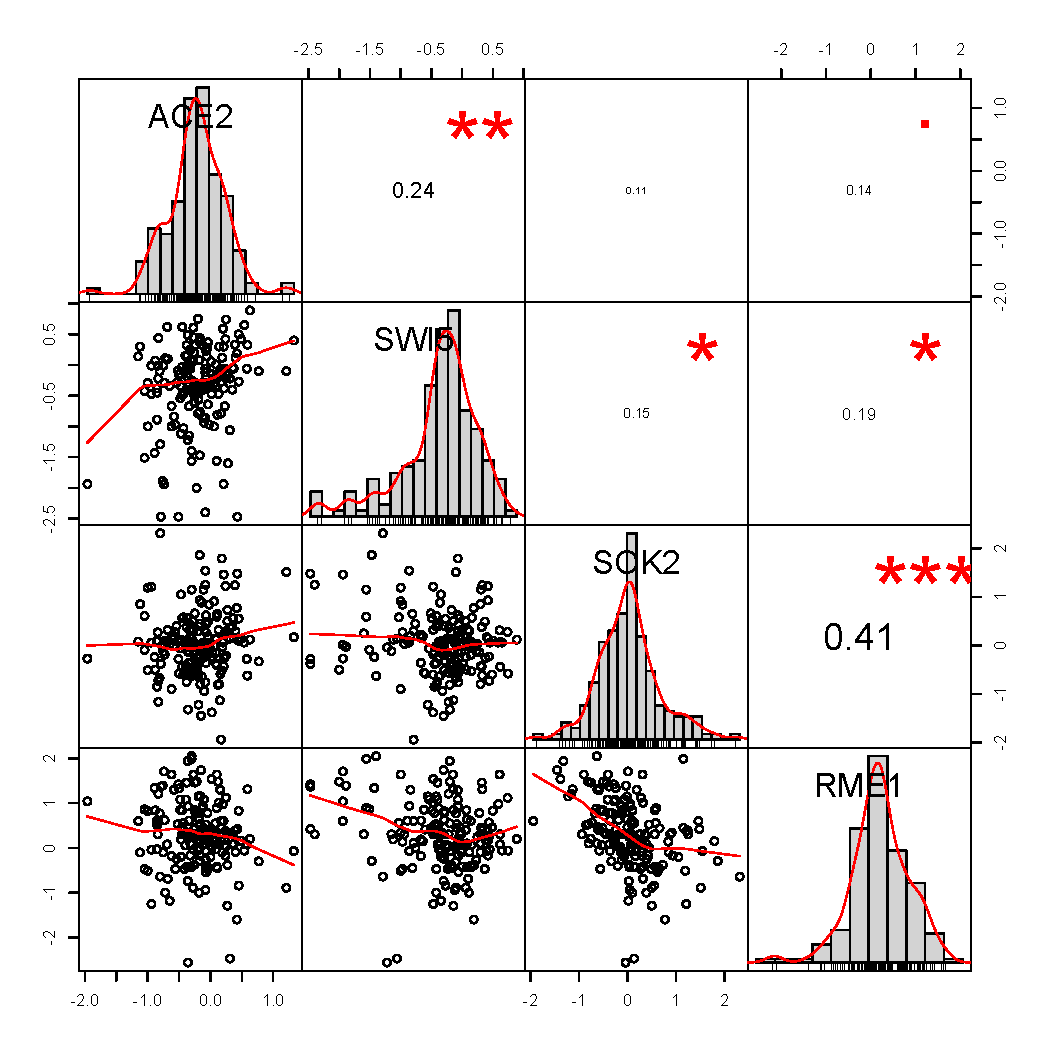
\includegraphics[width=0.5\columnwidth]{./figures/hands-on3/nice-pairs.pdf}
\caption{Output of the \lstinline!chart.Correlation()! function in the PerformanceAnalytics package, applied to the yeast expression data set.\label{fig:nicepairs}}
\end{figure}


% Here's an example based on code (see \href{http://gettinggeneticsdone.blogspot.com/2011/07/scatterplot-matrices-in-r.html}{this link} for the original source). Create a new R script called |mygraphs.R| and add the following function:
% %
% \begin{R}
% # panel.cor puts correlation in upper panels, size proportional to correlation
% panel.cor <- function(x, y, digits=2, prefix="", cex.cor, ...)
% {
%     usr <- par("usr"); on.exit(par(usr))
%     par(usr = c(0, 1, 0, 1))
%     r <- abs(cor(x, y))
%     txt <- format(c(r, 0.123456789), digits=digits)[1]
%     txt <- paste(prefix, txt, sep="")
%     if(missing(cex.cor))
%         cex.cor <- 0.8/strwidth(txt)
%     text(0.5, 0.5, txt, cex = cex.cor * r)
% }
% \end{R}
% You



\subsection{3D Scatter Plots}

A three-dimensional scatter plot can come in handy. The R library
\lstinline!lattice! has a function called \lstinline!cloud()! that
allows you to make such plots.
\begin{R}
> library(lattice)
> cloud(ACE2 ~ ASH1 * RAS2, data=yeast.clean)
> cloud(ACE2 ~ ASH1 * RAS2, data=yeast.clean, screen=list(x=-90, y=70)) # same plot from different angle
\end{R}
See the help file for \lstinline!cloud()! and \lstinline!panel.cloud()! for information on setting parameters.

\subsection{Scatterplot3D}
There is also a package available on CRAN called \lstinline!scatterplot3d! with similar functionality.
%
\begin{R}
> attach(yeast.clean) # so we can access the variables directly
> install.packages('scatterplot3d',dependencies=T) # installs scatterplot3d
> library(scatterplot3d) # assumes package is properly installed
> scatterplot3d(ASH1, RAS2, ACE2)
> scatterplot3d(ASH1, RAS2, ACE2, highlight.3d=T, pch=20,angle=25)
\end{R}
%
The |highlight.3d| argument colors points to help the viewer determine near and far points. Points that are closer to the viewer are lighter colors (more red in the default color scheme).

\subsubsection{Using Package Vignettes}
The Scatterplot3D package is quite flexible but this flexibility is hard to grok from the standard R help files (try |?scatterplot3d| to see for yourself).  Luckily the Scatterplot3D package includes a `vignette' -- a PDF document that discusses the design of the package and illustrates it's use.  Many packages include such vignettes. To see the list of vignettes available for your installed packages do the following:
%
\begin{R}
> vignette(all=T)
\end{R}
%
You should see that the vignette for the Scatterplot3D package is called |s3d|. You can access this vignette as follows, which should open the document in your default PDF viewer.
\begin{R}
> vignette("s3d")
\end{R}
%
In this case, the `good stuff' (i.e. the examples) starts on page 9 of the vignette.

\subsection{The rgl Package}

The 3D plots in |lattice| and |scatterplot3d| are fairly nice, but they don't allow the user to interact with the figures.  For example, wouldn't it be nice to be able to rotate a 3D scatter of points around to understand the relationships?  The |rgl| package allows you to do this, and can produce figures like that shown in Fig.~\ref{fig:rgl3d}.  Most R figures can be saved  using the |Save| option under the file menu. That's not the case for |rgl| plots. Instead we need to use the |rgl.postscript()| (creates a postscript or PDF version of the figure) or |snapshot3d()| (creates a screenshot) functions.
\begin{R}
> install.packages('rgl',dependencies=T)
> library(rgl)
> plot3d(ASH1, RAS2, ACE2, col='red', size=1, type='s')
> rgl.postscript('rgl3d-example.pdf', fmt='pdf')
\end{R}
%
\begin{figure}[htbp]
\centering
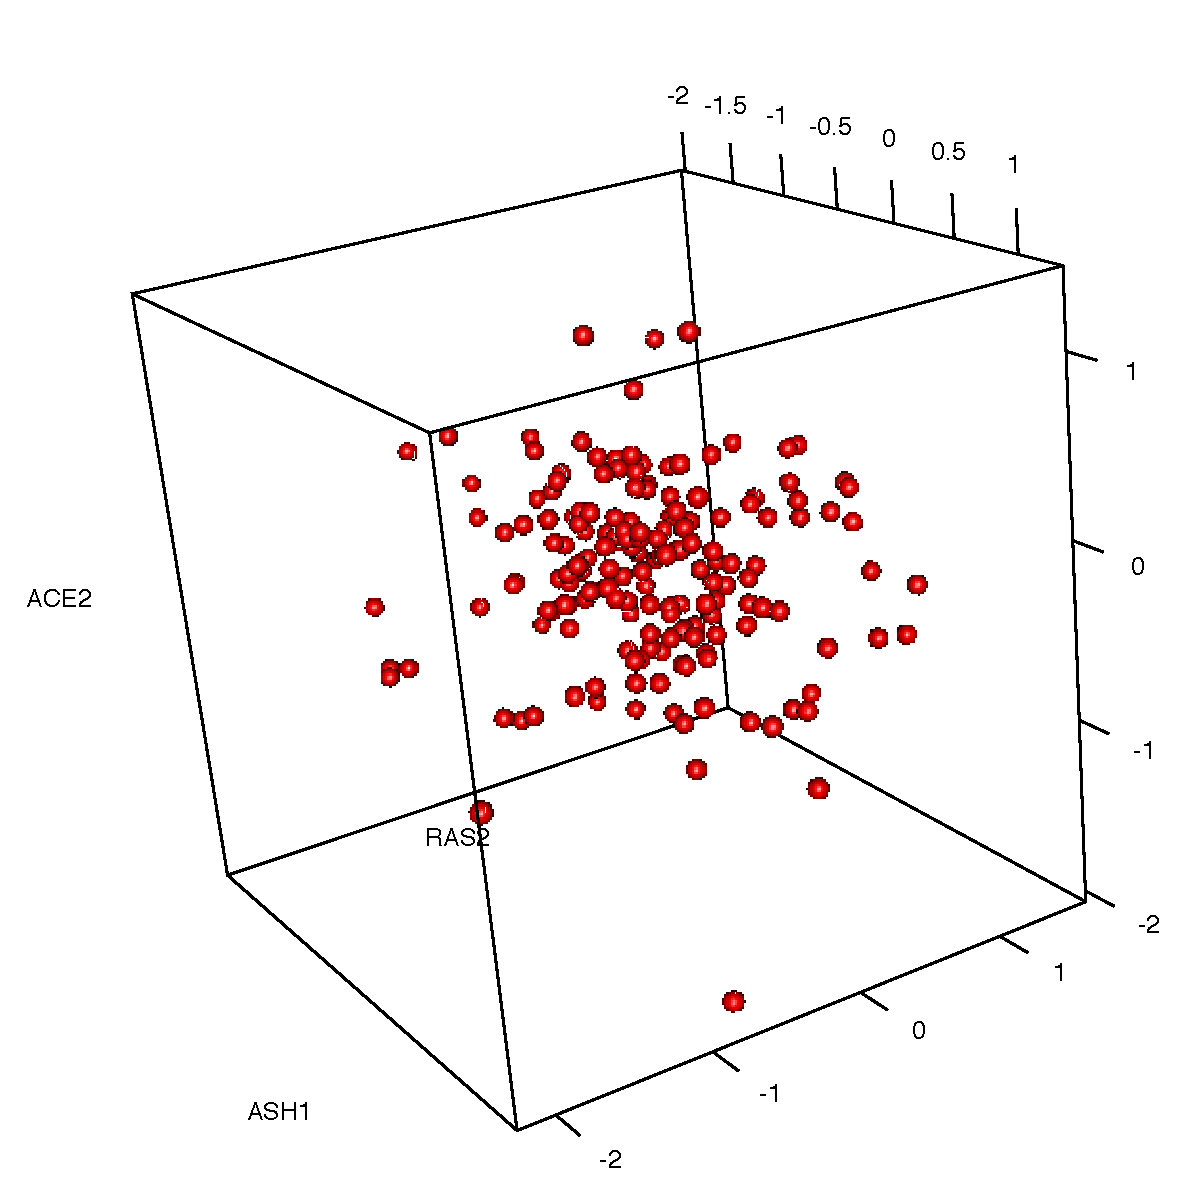
\includegraphics[width=0.5\columnwidth]{./figures/hands-on3/rgl3d-example.pdf}
\caption{Output of the \lstinline!plot3d()! function in the rgl package.\label{fig:rgl3d}}
\end{figure}

% Let's modify the 3D barplot on page 11 to create a 2D histogram. First we'll install another package -- |mvtnorm| -- that includes functions for creating multivariate normal distributions.
% %
% \begin{R}
% > install.packages('mvtnorm',dependencies=T)
% > library(mvtnorm)
% > ?rmvnorm # as always, check out the docs!

% \end{R}

\subsection{Colored grid plots}

A colored grid (or `heatmap') is another way of representing 3D data. It
most often is used to represent a variable of interest as a function of
two parameters. Grid plots can created using the \lstinline!image()!
function in R.

\begin{R}
> x <- seq(0, 2*pi, pi/20)
> y <- seq(0, 2*pi, pi/20)
> coolfxn <- function(x,y){
+    cos(x) * cos(y)}
> z <- outer(x,y,coolfxn) # the outer product of two matrices or vectors, see docs
> dim(z)
[1] 41 41
> image(x,y,z)
\end{R}
The \lstinline!x! and \lstinline!y! arguments to \lstinline!image()! are
vectors, the \lstinline!z! argument is a matrix (in this case created
using the outer product operator in conjunction with our function of
interest).

A somewhat more flexible function called |levelplot()| is found in the |lattice| package. For example, we can create a similar heatmap using |levelplot()| as follows:
\begin{R}
> library(lattice)
> levelplot(z)  # just the colors
> levelplot(z, contour=T) # colors plus contour lines
\end{R}
We can also apply the levelplot function to creat a representation of a correlation matrix, as shown here:
\begin{R}
> levelplot(cor(yeast.clean))
\end{R}
The default |levelplot()| colors are decent, but let's see how we can change the colors used to our liking. The |colorRampPalette()| function returns a function that interpolates between the values given as arguments to |colorRampPalette()|. So in the example below, it will create a series of colors from blue to white to red.
\begin{R}
> lvls <- seq(-1,1,0.1)  # set thresholds for our colors
> colors <- colorRampPalette(c('blue', 'white', 'red'))(length(lvls))
> levelplot(cor(yeast.clean), col.regions=colors, at=lvls)
\end{R}
%
The |colorRampPallete()| function can also take hexadecimal colors, as is commonly used in HTML. For a list of R colors see \url{http://research.stowers-institute.org/efg/R/Color/Chart/}.  For a  list of color schemes, developed by a geographer for effective cartographic representations,  see the \href{http://colorbrewer2.org/}{ColorBrewer web page}. For example, here's how to create the representation of the yeast data set correlation matrix shown in Fig.~\ref{fig:corrheat}:
\begin{R}
# this generates a color ramp from green to black to purple
> colors <- colorRampPalette(c('#1B7837', 'black', '#762A83'))(length(lvls))
> levelplot(cor(yeast.clean), col.regions=colors, at=lvls, scales=list(cex=0.6), xlab="", ylab="",main="Correlation Matrix\nYeast Expression Data")
\end{R}
The |scales| argument to |levelplot| changes the scaling of the tick marks and labels on the axes.

\begin{figure}[htbp]
\centering
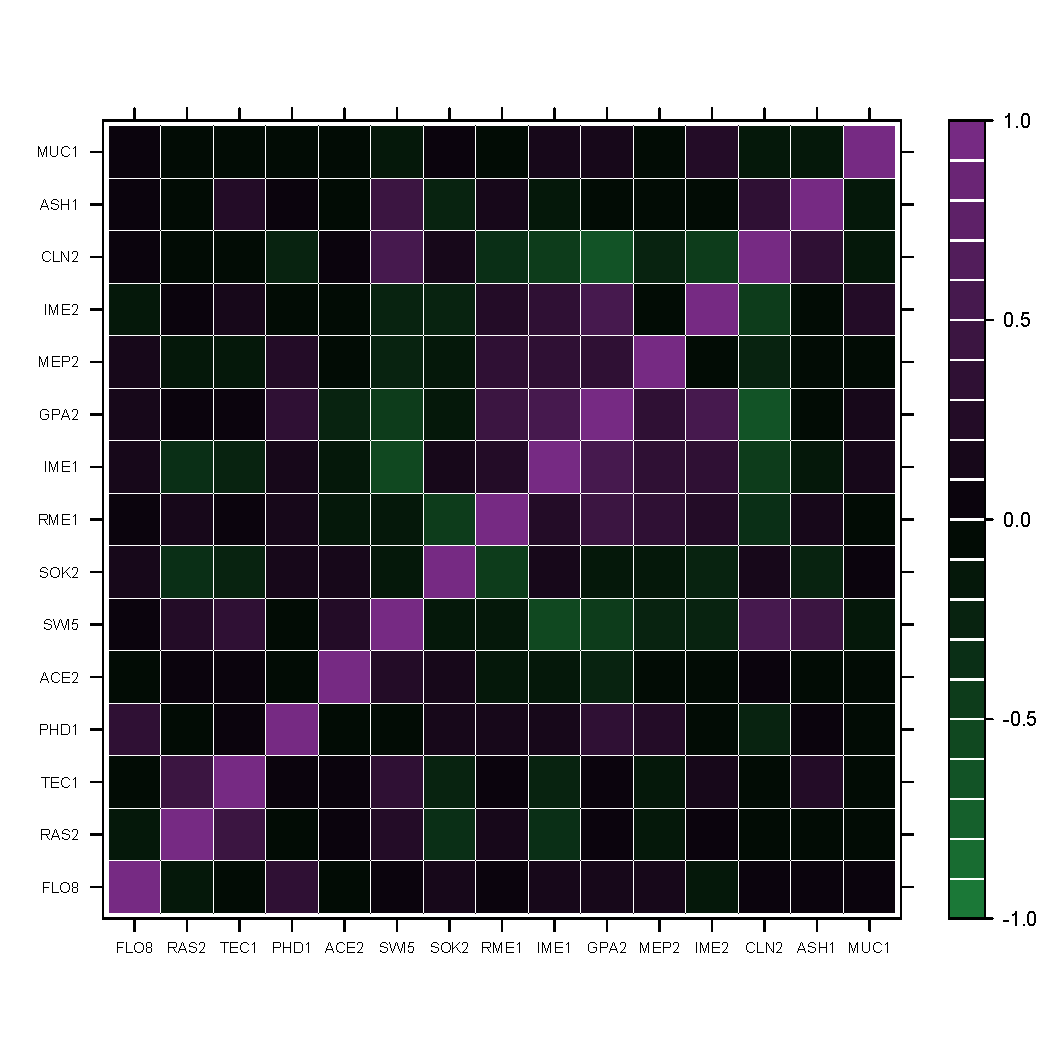
\includegraphics[width=0.5\columnwidth]{./figures/hands-on3/corr-heatmap.pdf}
\caption{A heatmap, representing the correlation matrix for the yeast expression data set, generated by the \lstinline!levelplot()! function in the lattice package.\label{fig:corrheat}}
\end{figure}


%
\section{Plotting in Python}

Python doesn't have any `native' data plotting tools but there are a
variety of packages that provide tools for visualizing data. The package
we're going to use is called `Matplotlib'. Matplotlib is one of the many
packages that is distributed with the Enthought Python distribution. If
you want to explore the full power of Matplotlib check out the example
gallery and the documentation at
\url{http://matplotlib.sourceforge.net/}.

\subsection{Basic plots using matplotib}

If you invoked the Ipython shell using the pylab option than most of the
basic matplotlib functions are already available to you. If not, import
them as so:

\begin{python}
>>> from pylab import *
>>> import numpy as np # go ahead and import numpy as well
\end{python}
\subsubsection{Loading data}

First let's load the yeast data set:

\begin{python}
>>> data = np.loadtxt('yeast-subnetwork-clean.txt',skiprows=1,usecols=range(1,16))
>>> data.shape   # check the dimensions of the resulting matrix
(173, 15)
\end{python}
The \lstinline!skiprows! argument tells the function how many rows in
the data file you want to skip. In this case we skipped only the first
row which gives the variable names. The \lstinline!usecols! arguments
specificies which columns from the data file to use. Here we skipped the
first (zeroth) column which had the names of the conditions. The usecols
\lstinline!loadtxt! works when there is no missing data. Use
\lstinline!numpy.genfromtxt! instead when there are missing values. For
a full tutorial on how to use the \lstinline!numpy.genfromtxt! function
see
\url{http://docs.scipy.org/doc/numpy/user/basics.io.genfromtxt.html}.

\subsubsection{Histograms in Matplotlib}

Matplotlib has a histogram drawing function. Here's how to use it:

\begin{python}
>>> hist? # in Ipython calls the help function
>>> h = hist(data[:,0]) # plot a histogram of the first variable (column) in our data set
>>> clf() # clear the plot window, don't need this if you closed the plot window
>>> h = hist(data[:,0], bins=20) # plot histogram w/20 bins
>>> h = hist(data[:,:2])  # histograms of the first two variables    
\end{python}
There's no built in density plot function, but we can create a function
that will do the necessary calculations for us to create our own density
plot. This uses a kernel density estimator function in the scipy library
(included with EPD). Put the following code in a file called
\lstinline!myplots.py! somewhere on your \lstinline!PYTHONPATH!:

\begin{python}
# myplots.py

import numpy as np
from scipy import stats

def density_trace(x):
    kde = stats.gaussian_kde(x)
    xmin,xmax = min(x), max(x)
    xspan = xmax - xmin
    xpts = np.arange(xmin, xmax, xspan/1000.)
    ypts = kde.evaluate(xpts) # evalude the estimate at the xpts
    return xpts,ypts
\end{python}
You can then use the \lstinline!density_trace! function as follows:

\begin{python}
>>> import myplots
>>> h = hist(data[:,0], normed=True) # use normed=True so histogram 
                           # is normalized to form a prob. density
>>> x,y = myplots.density_trace(data[:,0])
>>> plot(x,y, 'red')    
\end{python}
\subsubsection{Boxplots in Matplotlib}

Box-and-whisker plots are straightforward in Matplotlib:

\begin{python}
>>> b = boxplot(data[:,0])
>>> clf()
>>> b = boxplot(data[:,:5]) # boxplots of first 5 variables
\end{python}
The \lstinline!boxplot! function has quite a few facilities for
customizing your boxplots. For example, here's how we can create a
notched box-plot using 1000 bootstrap replicates (we'll discuss the
bootstrap in more detail in a later lecture) to calculate confidence
intervals for the median.

\begin{python}
>>> boxplot(data[:,0], notch=1, bootstrap=True)    
\end{python}
See the Matplotib docs for more info.

\subsubsection{Scatter Plots in Matplotlib}

Scatter plots are also easy to create:

\begin{python}
>>> s = scatter(data[:,0], data[:,1])    
\end{python}
\subsection{3D Plots}

Recent version of Matplotlib include facilities for creating 3D plots.
Here's an example of a 3D scatter plot:

\begin{python}
>>> from mpl_toolkits.mplot3d import Axes3D
>>> fig = figure()
>>> ax = fig.add_subplot(111, projection = '3d')
>>> ax.scatter(data[:,0],data[:,1],data[:,2])
<mpl_toolkits.mplot3d.art3d.Patch3DCollection object at 0x1a0bbd70>
>>> ax.set_xlabel('Gene 1')
<matplotlib.text.Text object at 0x1a0ae7d0>
>>> ax.set_ylabel('Gene 2')
<matplotlib.text.Text object at 0x1a0bb2b0>
>>> ax.set_zlabel('Gene 3')
<matplotlib.text.Text object at 0x1a0bbcd0>
>>> show()
\end{python}
Retyping all those commands is tedious and error prone so let's turn it
into a function. Add the following code to \lstinline!myplots.py!:

\begin{python}
from matplotlib import pyplot
from mpl_toolkits.mplot3d import Axes3D

def scatter3d(x,y,z, labels=None):
    fig = pyplot.figure()
    ax = fig.add_subplot(111, projection='3d')
    ax.scatter(x,y,z)

    if labels is not None:
        try:
            ax.set_xlabel(labels[0])
            ax.set_ylabel(labels[1])
            ax.set_zlabel(labels[2])
        except IndexError:
            print "You specificied less than 3 labels."
    return fig
\end{python}
Now reload myplots and call the scatter3d function as so:

\begin{python}
>>> reload(myplots)
>>> myplots.scatter3d(data[:,0], data[:,1], data[:,2])
>>> myplots.scatter3d(data[:,0], data[:,1], data[:,2], lab)
>>> myplots.scatter3d(data[:,0], data[:,1], data[:,2],labels=('X','Y','Z'))
\end{python}
\section{Plotting Geographic Data using Basemap}

There are a number of toolkits available for Matplotlib that extend the
functionality of the package. The mplot3d is one of those toolkits which
has now been incorporated into the standard distribution. Basemap is
another toolkit that provides the ability to plot 2D data on maps. The
Basemap toolkit supports a variety of mapping projections and coordinate
transformations and has the ability to plot things likes water bodies
and political boundaries.

The EPD edition of Python includes Basemap but in the interest of space
they have removed the high resolution maps that the normal Basemap
distribution includes. In order to use those maps you can download a
basemap binary (for Windows) or the source code (on OS X) from the
\href{http://sourceforge.net/projects/matplotlib/files/matplotlib-toolkits/basemap-1.0.1/}{here}.

On Windows just run the executable installer (make sure you get the
version that is appropriate to your EPD distribution; either 32-bit or
64-bit).

On OS X, once you have downloaded the source tarball
(\lstinline!basemap-1.0.1.tar.gz!), open up a bash shell, navigate to
the directory where you saved the tarball, and type:

\begin{python}[language=bash]
tar xvzf basemap-1.0.1.tar.gz
\end{python}
This will decompress and unarchive the source code into a directory
called \lstinline!basemap-1.0.1!. Navigate to the directory where the
mapping data is stored:

\begin{python}[language=bash]
cd basemap-1.0.1/lib/mpl_toolkits/basemap/data
\end{python}
And then copy all the \lstinline!.dat! files to your Python
installation:

\begin{python}[language=bash]
cp *.dat /Library/Frameworks/Python.framework/Versions/Current/lib/python2.7/site-packages/mpl_toolkits/basemap/data
\end{python}
\subsection{Using Basemap}

In our first basemap example we show how to plot the US lower 48 and we
add a red dot to represent the city of Durham, NC. Save this code as
\lstinline!mapex.py! and run it from the command line
(\lstinline!python mapex.py!).

\begin{codeblock}[python]
# Derived from: Tosi, Sandro. Plotting Geographical Data using Basemap
# url: http://www.packtpub.com/article/plotting-geographical-data-using-basemap

import numpy as np
from matplotlib import pyplot
from mpl_toolkits.basemap import Basemap

# Lambert Conformal map of USA lower 48 states
m = Basemap(llcrnrlon=-119, llcrnrlat=22, urcrnrlon=-64,
  urcrnrlat=49, projection='lcc', lat_1=33, lat_2=45,
  lon_0=-95, resolution='l', area_thresh=10000)

# draw the coastlines of continental area
m.drawcoastlines()
# draw country boundaries
m.drawcountries(linewidth=2)
# draw states boundaries (America only)
m.drawstates()

# fill the background (the oceans)
m.drawmapboundary(fill_color='aqua')
# fill the continental area and lakes
m.fillcontinents(color='coral',lake_color='aqua')

# draw pt. indicating durham/raleigh area
# Durham, latitude:  35deg 52min N, longitude:78deg 47min W
dlat, dlong = 35.86, -78.78 # west is minus

# this maps latitude and longitude to map coordinates
mcoordx, mcoordy = m(dlong,dlat)
pyplot.plot(mcoordx,mcoordy, 'ro') # draw red dot
pyplot.text(mcoordx+36000, mcoordy-18000, 'Durham')

# finally show the file
pyplot.show()    
\end{codeblock}
%
In our second example let's assume you've been studying the population
genetics of the beautiful and rare North Carolina Blue Snouter (mammals
of the order Rhinogradentia; see Stümpke 1967. The snouters: form and
life of the Rhinogrades). You've been sampling snouter populations from
across NC and you want to make a figure for a paper showing all your
sampling locations. Download the file \lstinline!nc-sites.txt! from the
course wiki, and place it in the same directory as the following module
(\lstinline!mapex2.py!).

\begin{codeblock}[python]
# mapex2.py

import numpy as np
from matplotlib import pyplot
from mpl_toolkits.basemap import Basemap

m = Basemap(llcrnrlon=-85, llcrnrlat=33, urcrnrlon=-75,
  urcrnrlat=37, projection='lcc', lat_0=35.774, lon_0=-78.634,
  resolution='l', area_thresh=10000)

m.drawcoastlines()
m.drawcountries(linewidth=2)
m.drawstates()
m.drawmapboundary(fill_color='aqua')
m.fillcontinents(color='coral',lake_color='aqua')

sites = np.loadtxt('nc-sites.txt')

for row in sites:
    lat, lon = row[0], row[1]
    x,y = m(lon, lat) # note how longitude (x-direction) comes first
    # use blue +'s to plot sites
    pyplot.plot(x,y, 'b+', markersize=8,markeredgewidth=2) 

pyplot.show()    
\end{codeblock}
%
The \lstinline!mapex2.py! code will produce a figure like the one below.

\begin{figure}[htbp]
\centering
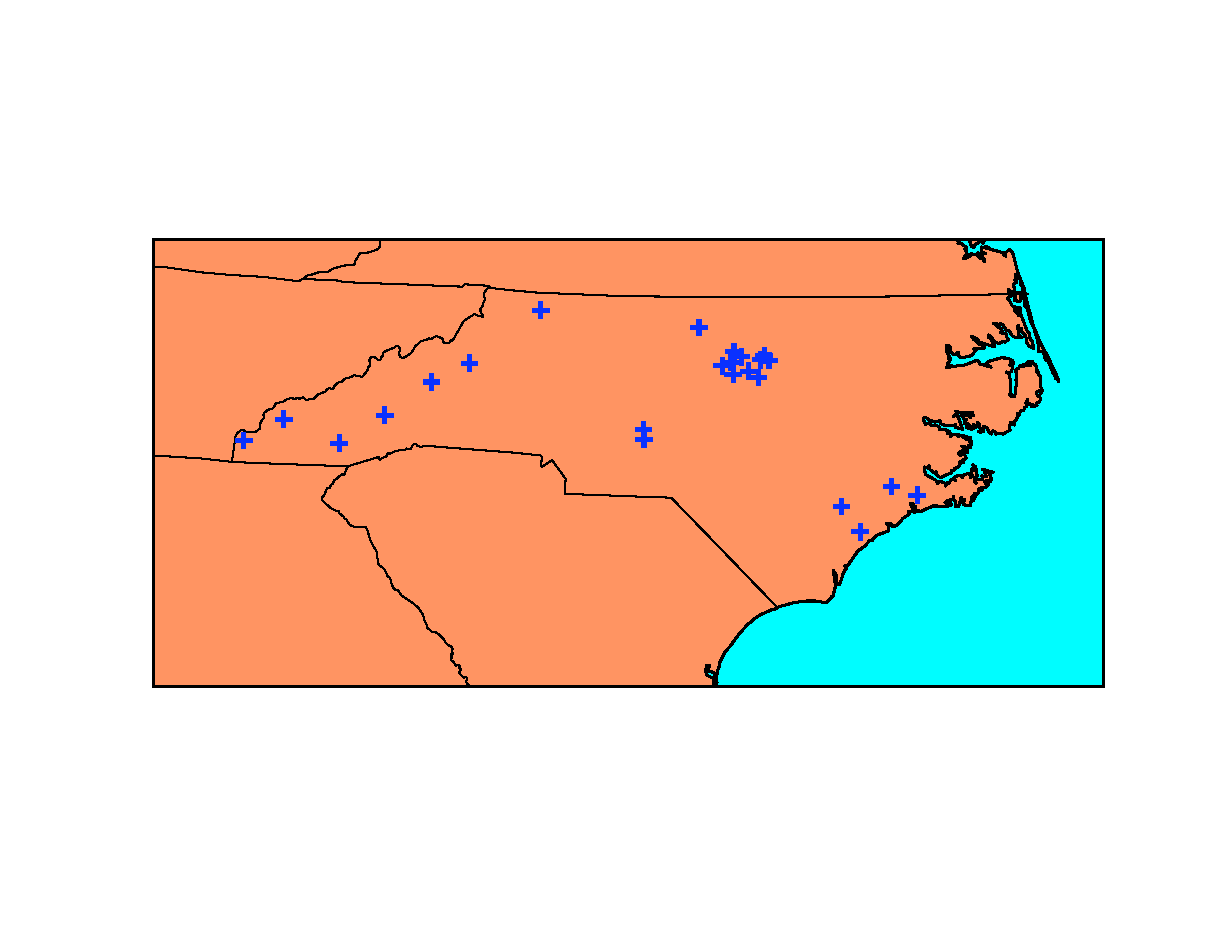
\includegraphics[width=0.6\columnwidth]{./figures/hands-on3/mapfig.pdf}
\caption{Output of the mapex2.py module}
\end{figure}






% \chapter{Multiple Regression in R}
% 

\section{Multiple Regression in R}

To illustrate multiple regression in R we'll use a built in dataset called |trees|. |trees| consists of measurements of the girth, height, and volume of 31 black cherry trees (|?trees| for more info). We'll start with some summary tables and diagnostic plots to familiarize ourselves with the data:
%
\begin{R}
> names(trees)
[1] "Girth"  "Height" "Volume"
> dim(trees)
[1] 31  3
> summary(trees)
     Girth           Height       Volume
 Min.   : 8.30   Min.   :63   Min.   :10.20
 1st Qu.:11.05   1st Qu.:72   1st Qu.:19.40
 Median :12.90   Median :76   Median :24.20
 Mean   :13.25   Mean   :76   Mean   :30.17
 3rd Qu.:15.25   3rd Qu.:80   3rd Qu.:37.30
 Max.   :20.60   Max.   :87   Max.   :77.00

# we'll use the chart.Correlation fxn that we introduced last week 
> library(PerformanceAnalytics)  
> chart.Correlation(trees)
\end{R}
%
As one might expect, the scatterplot matrix shows that all the variables are positively correlated, and girth and volume have a  particularly strong correlation.

Let's assume we're lumberjacks, but our permit only allows us to harvest a fixed number of trees.  We get paid by the total volume of wood we harvest, so we're interested in predicting a tree's volume (hard to measure directly) as a function of its girth and height (relatively easy to measure), so we can pick the best trees to harvest.  We'll therefore calculate a multiple regression of volume on height and width. Let's start by taking a look at the 3D scatter of the data using the plot3d function from the |rgl| package.
%
\begin{R}
> library(rgl)
> plot3d(trees, col='red', size=1, type='s') # use your mouse to rotate the plot
\end{R}
%
From the 3D scatter plot it looks like we ought to be able to find a plane through the data that fits the scatter fairly well. Let's use the |lm()| function to calculate the multiple regression:
%
\begin{R}
> l <- lm(Volume ~ Girth + Height, data=trees)
\end{R}
%
To visualize the multiple regression, let's use the |scatterplot3d| package to draw the 3D scatter of plots and the plane that corresponds to the regression model:
%
\begin{R}
> library(scatterplot3d)  # install this package first if needed
> p <- scatterplot3d(trees,angle=55,type='h')
> title('Tree Volume as\na function of Girth and Height')
> p$plane3d(l, col='orangered')
> dev.copy(pdf, 'trees-regrfit.pdf')  # copy plot to a pdf file
> dev.off()  # write the file
\end{R}
%
Notice the use of |dev.copy()| and |dev.off()| to save the plot from the console.  The output this generates should look similar to Fig.~\ref{fig:treesregr}.
%
\begin{figure}[htbp]
\centering
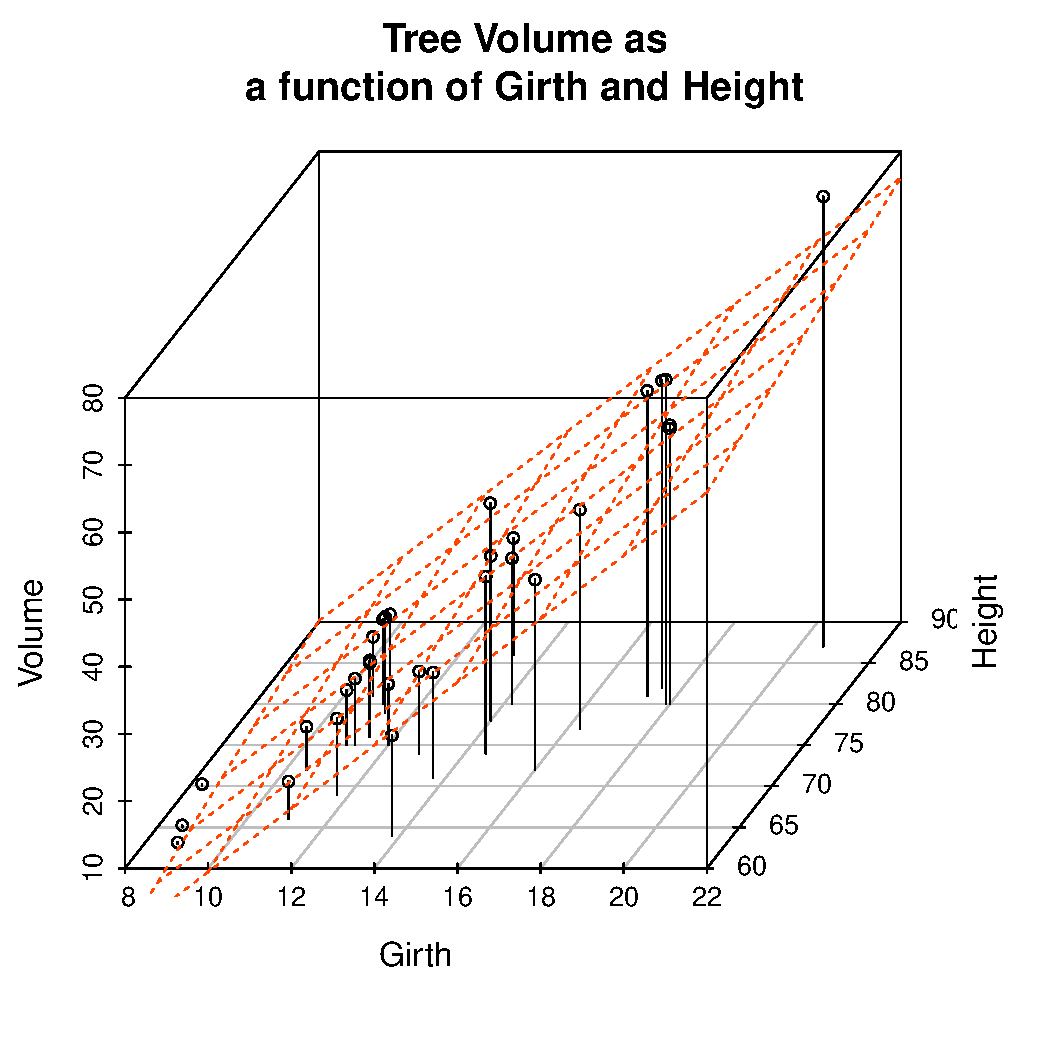
\includegraphics[width=0.5\columnwidth]{./figures/hands-on4/trees-regrfit.pdf}
\caption{Multiple regression plot of cherry tree volume on girth and height, generated using the \texttt{scatterplot3d} library\label{fig:treesregr}}
\end{figure}

From the figure it looks like the regression model fits pretty well, as we anticipated  from the pairwise relationships.  Let's use the |summary()| function to obtain details of the model:
\begin{R}
> summary(l)

Call:
lm(formula = Volume ~ Girth + Height, data = trees)

Residuals:
    Min      1Q  Median      3Q     Max
-6.4065 -2.6493 -0.2876  2.2003  8.4847

Coefficients:
            Estimate Std. Error t value Pr(>|t|)
(Intercept) -57.9877     8.6382  -6.713 2.75e-07 ***
Girth         4.7082     0.2643  17.816  < 2e-16 ***
Height        0.3393     0.1302   2.607   0.0145 *
---
Signif. codes:  0 ‘***’ 0.001 ‘**’ 0.01 ‘*’ 0.05 ‘.’ 0.1 ‘ ’ 1

Residual standard error: 3.882 on 28 degrees of freedom
Multiple R-squared: 0.948,  Adjusted R-squared: 0.9442
F-statistic:   255 on 2 and 28 DF,  p-value: < 2.2e-16
\end{R}
%
The regression equation is: $\hat{y} = 4.71x_1 + 0.34x_2$, where $y$ is Volume, and $x_1$ and $x_2$ are Girth and Height respectively. Since they're on different scales the coefficients for Girth and Height aren't directly comparable. Both coefficients are significant at the $p<0.05$ level, but note that Girth is the much stronger predictor. In fact the addition of height explains only a minor additional fraction of variation in tree volume, so from the lumberjack's perspective the additional trouble of measuring height probably isn't worth it.

\subsection{Exploring the Vector Geometry of a Regression Model}

The object returned by the |lm()| function hold lots of useful information:
%
\begin{R}
> names(l)
 [1] "coefficients"  "residuals"     "effects"       
     "rank"          "fitted.values" "assign"
 [7] "qr"            "df.residual"   "xlevels" 
     "call"          "terms"         "model"
\end{R}
%
The |fitted.values| correspond to the predicted values of the outcome variable ($\hat{y}$). Let's use our knowledge of vector geometry to further explore the relationship between the predicted Volume and the predictor variables.  By definition the vector representing the predicted values lies in the plane defined by Height and Girth, so let's do some simple calculations to understand their length and angular relationships:
%
\begin{R}
# proportional to length of vectors
> sd(l$fitted.values)
[1] 16.00434
> sd(trees$Height)
[1] 6.371813
> sd(trees$Girth)
[1] 3.138139

# cosines of angles btw vectors
> cor(trees$Height, trees$Girth)
[1] 0.5192801
> cor(trees$Height, l$fitted.values)
[1] 0.6144545
> cor(trees$Girth, l$fitted.values)
[1] 0.9933158

# angles btw vectors in degrees
> acos(cor(trees$Height, l$fitted.values)) * (180/pi)
[1] 52.08771
> acos(cor(trees$Girth, l$fitted.values)) * (180/pi)
[1] 6.628322
> acos(cor(trees$Girth, trees$Height)) * (180/pi)
[1] 58.71603
\end{R}
%

\begin{tcolorbox}[title=In class assignment]
Using the calculations above you should now be able to sketch out by hand, a diagram depicting the vector relationships between Height, Girth, and the predicted Volume .  Once you've finished with your sketch, discuss it with your fellow classmates.  Did you get similar answers? If not, discuss it and try to come up with an agreed upon representation.
\end{tcolorbox}

\subsection{Exploring the Residuals from the Model Fit}

Now let's look at the residuals from the regression. The residuals represent the `unexplained' variance:
\begin{R}
> plot(trees$Volume,l$residuals, xlab='Volume',ylab='Regression Residuals')
> abline(h=0, lty='dashed', col='red')
\end{R}
%
Ideally the residuals should be evenly scattered around zero, with no trends as we go from high to low values of the dependent variable.  As you can see in Fig.~\ref{fig:trees-resid} it looks like that the residuals on the left tend to be below zero, while those on the far right of the plot are consistently above zero, suggesting that there may be a non-linear aspect of the relationship that our model isn't capturing.
%
\begin{figure}[htbp]
\centering
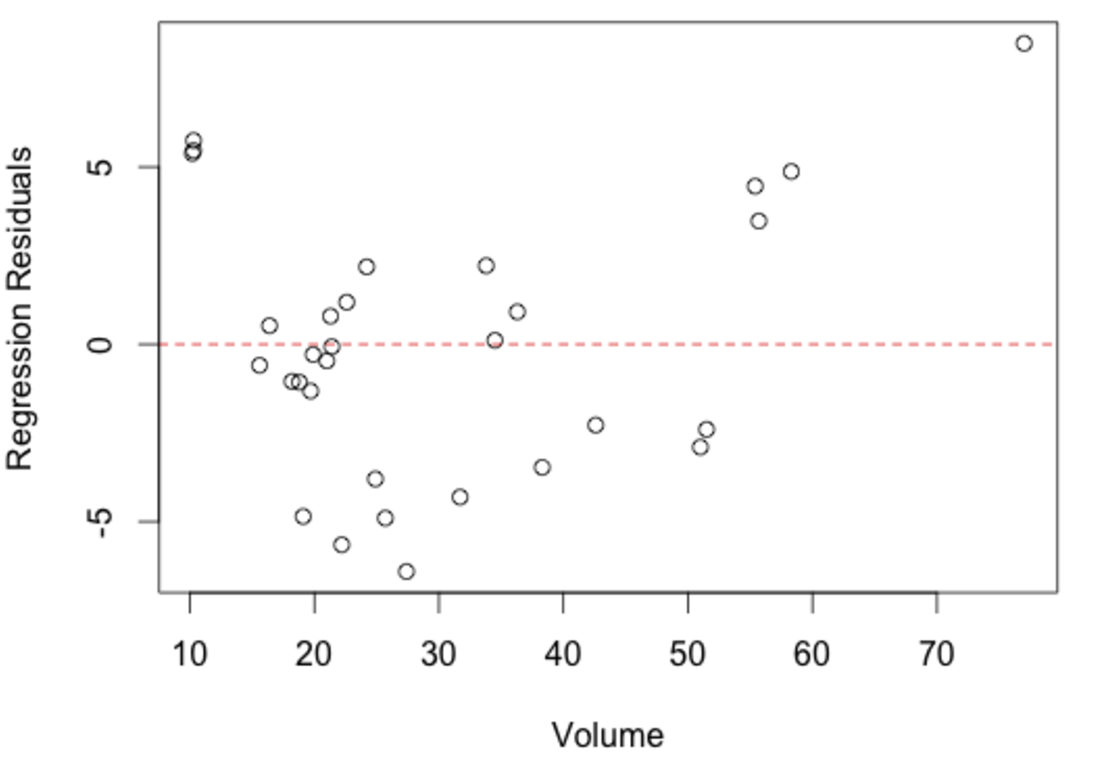
\includegraphics[height=1.5in]{./figures/hands-on4/trees-residuals.pdf}
\caption{Residual plot based on the multiple regression plot of cherry tree volume on girth and height,\label{fig:trees-resid}}
\end{figure}

Let's think about the relationships we're actually modeling for a few minutes.  For the sake of simplicity let's consider the trunk of a tree to be a cylinder.  How do the dimensions of this cylinder relate to its volume? You can look up the formula for the volume of a cylinder, but the key thing you'll want to note is that volume of the cylinder should be proportional to a characteristic length of the cylinder cubed ($V \propto \mathrm{L}^3$). This suggests that if we want to fit a linear model we should relate Girth to $\sqrt[3]{\mathrm{Volume}}$. Let's explore this a little. Since our initial multiple regression suggested that height had relatively little predictive power, we'll simplify our model down to a single predictor:
%
\begin{R}
> cuberoot.V <- trees$Volume^0.33
> cor(trees$Volume, trees$Girth)
[1] 0.9671194
> cor(cuberoot.V, trees$Girth)
[1] 0.9777078
> l.orig <- lm(trees$Volume~ trees$Girth)
> l.transf <- lm(cuberoot.V ~ trees$Girth)
> summary(l.orig)

Call:
lm(formula = trees$Volume ~ trees$Girth)

Residuals:
   Min     1Q Median     3Q    Max
-8.065 -3.107  0.152  3.495  9.587

Coefficients:
            Estimate Std. Error t value Pr(>|t|)
(Intercept) -36.9435     3.3651  -10.98 7.62e-12 ***
trees$Girth   5.0659     0.2474   20.48  < 2e-16 ***
---
Signif. codes:  0 ‘***’ 0.001 ‘**’ 0.01 ‘*’ 0.05 ‘.’ 0.1 ‘ ’ 1

Residual standard error: 4.252 on 29 degrees of freedom
Multiple R-squared: 0.9353, Adjusted R-squared: 0.9331
F-statistic: 419.4 on 1 and 29 DF,  p-value: < 2.2e-16

> summary(l.transf)

Call:
lm(formula = cuberoot.V ~ trees$Girth)

Residuals:
     Min       1Q   Median       3Q      Max
-0.18919 -0.09775 -0.01488  0.07855  0.26427

Coefficients:
            Estimate Std. Error t value Pr(>|t|)
(Intercept)  0.82543    0.08856   9.321 3.18e-10 ***
trees$Girth  0.16324    0.00651  25.076  < 2e-16 ***
---
Signif. codes:  0 ‘***’ 0.001 ‘**’ 0.01 ‘*’ 0.05 ‘.’ 0.1 ‘ ’ 1

Residual standard error: 0.1119 on 29 degrees of freedom
Multiple R-squared: 0.9559, Adjusted R-squared: 0.9544
F-statistic: 628.8 on 1 and 29 DF,  p-value: < 2.2e-16
\end{R}
%
Comparing the summary tables, we see indeed that using the cube root of Volume improves the fit of our model some. Let's examine the residuals.
%
\begin{R}
> layout(c(1,2), widths=c(3,3), heights=c(2,2))
> plot(trees$Volume, l.orig$residuals, xlab='Volume', ylab="Residuals")
> abline(h = 0, col='red', lty='dashed')
> plot(cuberoot.V, l.transf$residuals, 
        xlab='Volume^0.33', ylab='Residuals')

> abline(h = 0, col='red', lty='dashed')
> dev.copy(pdf, 'compare-residuals.pdf')
> dev.off()
> layout(c(1,1))   # reset the layout
\end{R}
%
\begin{figure}[htbp]
\centering
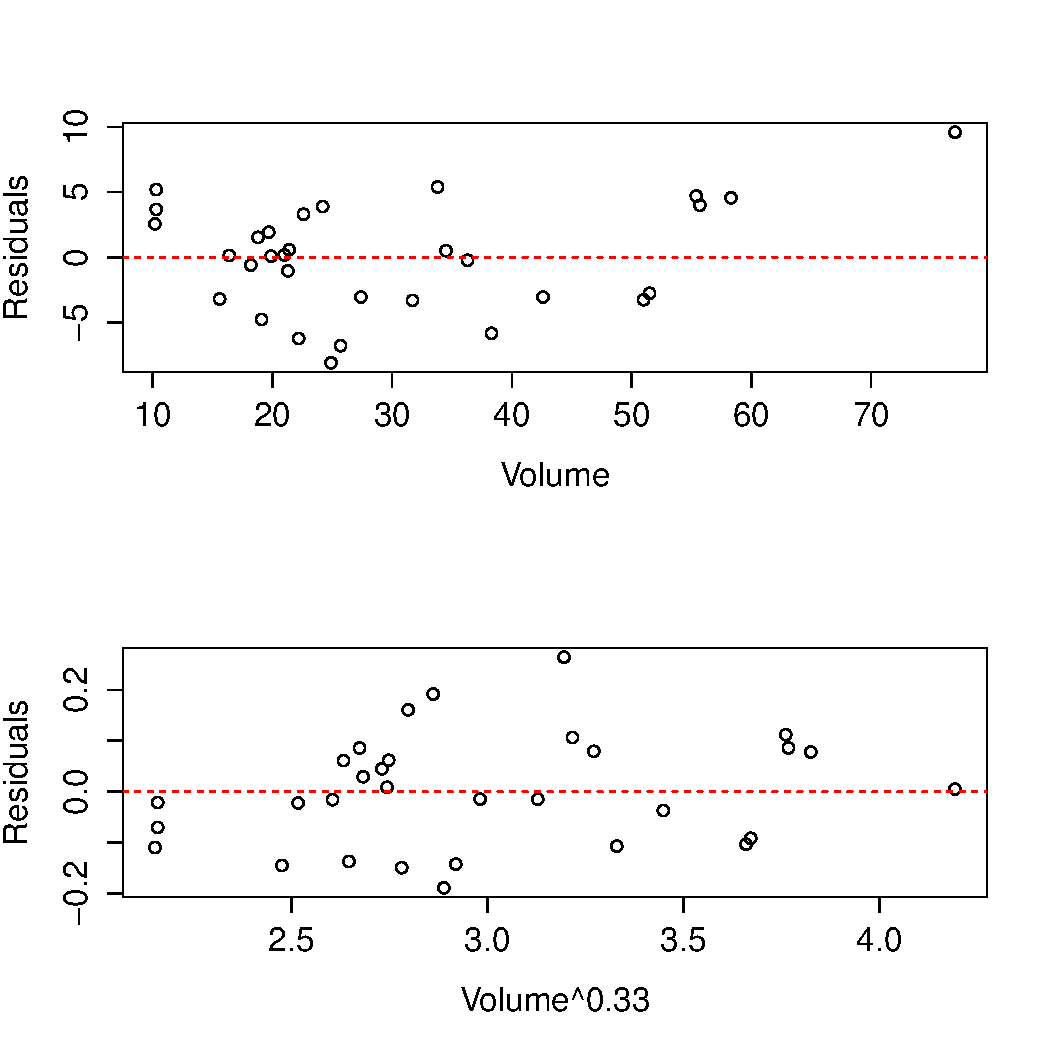
\includegraphics[height=2in]{./figures/hands-on4/compare-residuals.pdf}
\caption{Residual plot based on the bivariate regression of tree volume on girth, or $\sqrt[3]{V}$ on girth \label{fig:compare-resid}}
\end{figure}
%
As we can see the transformation we applied to the data did seem to make our residuals more uniform across the range of observations. Note the use of the |layout()| function to put multiple plots in the same figure.

\subsection{Fitting a curvilinear model using lm()}

Above we transformed the volume data in order to fit a straight line relationship between $\sqrt[3]{V}$  and Girth. However, we could just as easily have applied a cubic regression to the original variables as shown below (remember this is still linear  in the coefficients):

\begin{R}
> lm.3 <- lm(Volume ~ I(Girth^3), data=trees)
> summary(lm.3)

Call:
lm(formula = Volume ~ I(Girth^3), data = trees)

Residuals:
   Min     1Q Median     3Q    Max
-4.526 -3.036  0.215  2.419  8.291

Coefficients:
             Estimate Std. Error t value Pr(>|t|)
(Intercept) 8.0426960  1.0426698   7.714 1.66e-08 ***
I(Girth^3)  0.0081365  0.0003118  26.098  < 2e-16 ***
---
Signif. codes:  0 ‘***’ 0.001 ‘**’ 0.01 ‘*’ 0.05 ‘.’ 0.1 ‘ ’ 1

Residual standard error: 3.379 on 29 degrees of freedom
Multiple R-squared: 0.9592, Adjusted R-squared: 0.9578
F-statistic: 681.1 on 1 and 29 DF,  p-value: < 2.2e-16

> lm.3$coefficients
(Intercept)  I(Girth^3)
8.042696007 0.008136533
> a0 = lm.3$coefficients[[1]]
> B1 = lm.3$coefficients[[2]]
> x <- seq(8,25,0.25) # range of values to evaluate model over
> fit <- a0 + B1*x^3
> plot(Volume ~ Girth, data=trees)
> lines(x,fit,col='red')
> figtext <- paste(c("Volume = ", round(a0,2), "+", round(B1,4), "*Girth^3"), collapse='')
> text(12, 60, figtext)
\end{R}
%
\begin{figure}[htbp]
\centering
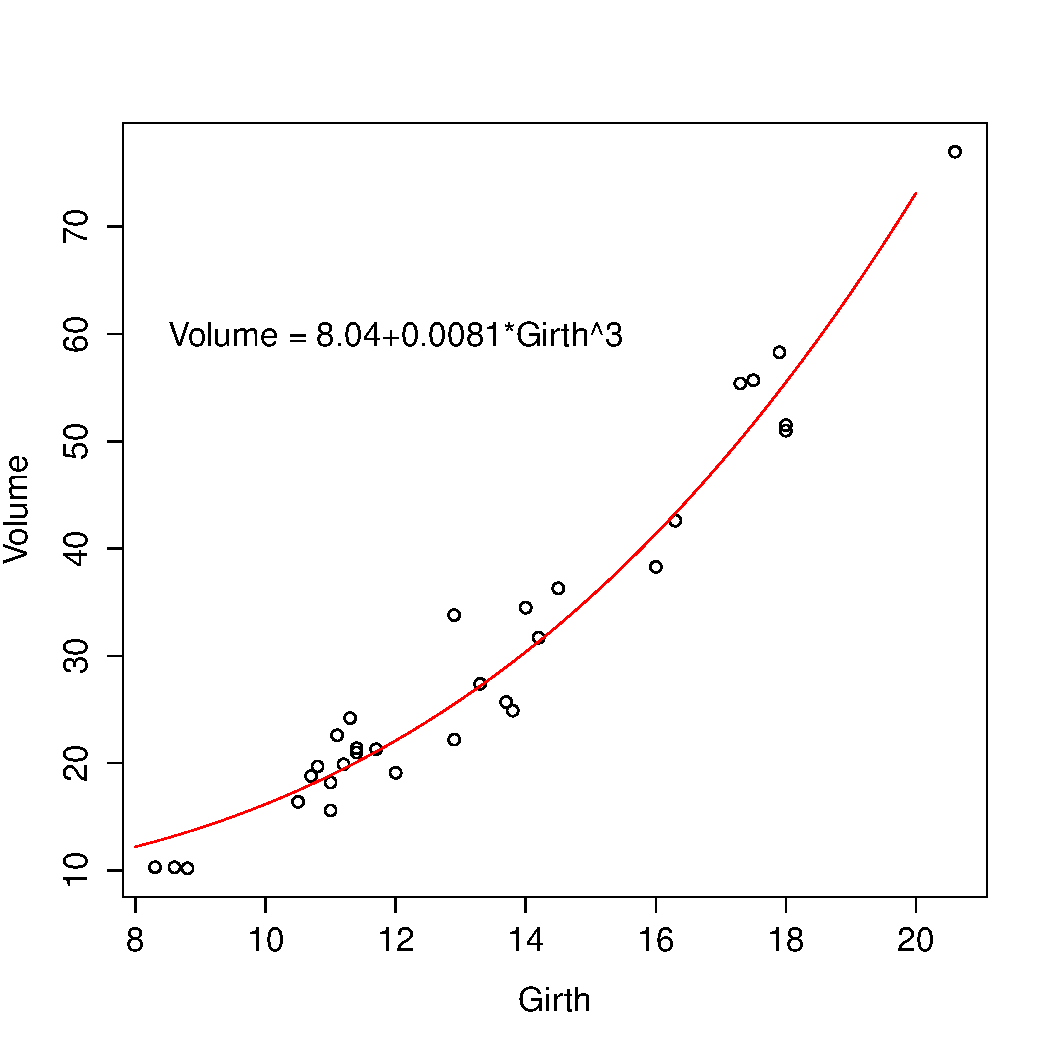
\includegraphics[height=2in]{./figures/hands-on4/cubic-regr.pdf}
\caption{Cubic regression of tree volume on girth \label{fig:cubic-regr}}
\end{figure}
%
The |I()| function used above requires a little explanation.  Normally, the R formula syntax (see |?formula|) treats the carat symbol, |'^'|, as short-hand for factor crossing to the specified degree.  For example, the formula |(a+b+c)^2| would be interpretted as the model with main effects and all second order interaction terms, i.e. |a + b + c + a:b + a:c + b:c| where the colons indicate interactions.  The |I()| function `protects' the object in it's argument; in this case telling the regression function to treat this as Girth raised to the third power as opposed to trying to construct interaction terms for Girth.


\medskip
\begin{assignment}
Write a function, |mult.regr(X,y)| that calculates the multiple regression of $y$ on multiple predictors, $x_1, x_2, \ldots x_k$ \emph{using matrix operations}. Your function should take two arguments, |X| and |y|, where |X| is a matrix representing the predictor variables and |y| is a vector for the outcome variable.  Your function should return a list containg the vector of regression coeffients, $B$, the coefficient of determination ($R^2$), and a vector, $\hat{y}$, representing the fitted values.  Refer to the slides from lecture 4 (and possibly lecture 2 if you need a refresher) to review the matrix  solution to the regression problem.
\end{assignment}


\section{Exploring the impact of nearly collinear predictors on regression}

In lecture we discussed the problems that can arise in regression when your predictor variables are nearly collinear. In this section we'll illustrate some of these issues.

Consider again the |trees| data set.  Recall that two of the variables -- Girth and Volume -- are highly correlated and thus nearly collinear.
%
\begin{R}
> cor(trees)
           Girth    Height    Volume
Girth  1.0000000 0.5192801 0.9671194
Height 0.5192801 1.0000000 0.5982497
Volume 0.9671194 0.5982497 1.0000000
\end{R}
%
Let's explore what happens when we treat Height as the dependent variable, and Girth and Volume as the predictor variables.
%
\begin{R}
> lm.H <- lm(Height ~ Girth + Volume, data = trees)
> summary(lm.H)

Call:
lm(formula = Height ~ Girth + Volume, data = trees)

Residuals:
    Min      1Q  Median      3Q     Max 
-9.7855 -3.3649  0.5683  2.3747 11.6910 

Coefficients:
            Estimate Std. Error t value Pr(>|t|)    
(Intercept)  83.2958     9.0866   9.167 6.33e-10 ***
Girth        -1.8615     1.1567  -1.609   0.1188    
Volume        0.5756     0.2208   2.607   0.0145 *  
---
Signif. codes:  0 ‘***’ 0.001 ‘**’ 0.01 ‘*’ 0.05 ‘.’ 0.1 ‘ ’ 1

Residual standard error: 5.056 on 28 degrees of freedom
Multiple R-squared:  0.4123,    Adjusted R-squared:  0.3703 
F-statistic:  9.82 on 2 and 28 DF,  p-value: 0.0005868
\end{R}
%
We can, of course, fit the linear model despite the collinearity, and we find that the model does have some predictive power, with $R^2 = 0.41$, and with Volume being the more significant predictor.

Now, let's created a slightly different version of the trees data set by add some noise to the three variables.   Our goal here is to simulate a data set we might have created had we measured a slightly different set of trees during our sampling. We'll use the |jitter| function to add uniform noise to the data set.
%
\begin{R}
> jitter.Girth <- jitter(trees$Girth, amount= 0.25 * sd(trees$Girth))
> jitter.Height <- jitter(trees$Height, amount= 0.25 * sd(trees$Height))
> jitter.Volume <- jitter(trees$Volume, amount= 0.25 * sd(trees$Volume))
> jitter.trees <- data.frame(Girth = jitter.Girth, 
                        Height = jitter.Height, 
                        Volume = jitter.Volume)
\end{R}
%
Here we added uniform noise proportional to the one-quarter the standard deviation of each variable.  Let's take a moment to convince ourselves that our new data set, |jitter.trees|, is not too different from the |trees| data set from which it was derived.
%
\begin{R}
# compare this to summary(trees)
# You will get slightly different answers because jitter adds random noise

> summary(jitter.trees)
     Girth            Height          Volume     
 Min.   : 7.913   Min.   :62.31   Min.   :10.75  
 1st Qu.:10.971   1st Qu.:72.37   1st Qu.:18.99  
 Median :12.606   Median :76.54   Median :22.38  
 Mean   :13.170   Mean   :75.84   Mean   :29.77  
 3rd Qu.:15.183   3rd Qu.:80.63   3rd Qu.:37.71  
 Max.   :20.722   Max.   :85.91   Max.   :77.69  

# correlations among jittered variables are
# similar to those of the original variables

> cor(jitter.trees)
           Girth    Height    Volume
Girth  1.0000000 0.4924240 0.9433214
Height 0.4924240 1.0000000 0.5531763
Volume 0.9433214 0.5531763 1.0000000    

## jittered variables are highly correlatd with original variables

> cor(trees$Height, jitter.trees$Height)
[1] 0.9861006
> cor(trees$Girth, jitter.trees$Girth)
[1] 0.9928097
> cor(trees$Volume, jitter.trees$Volume)
[1] 0.9883385

> plot(trees$Height, jitter.trees$Height)
> plot(trees$Girth, jitter.trees$Girth)
> plot(trees$Volume, jitter.trees$Volume)
\end{R}

Now that we've convinced ourselves that our jittered data set is a decent approximation to our original data set, let's re-calculate the linear regression, and compare the coefficients of the jittered model to the original model:
%
\begin{R}
> lm.H.jitter <- lm(Height ~ Girth + Volume, data = jitter.trees)
> coefficients(lm.H.jitter)
(Intercept)       Girth      Volume 
 73.3492169  -0.5437115   0.3241854 
> coefficients(lm.H)
(Intercept)       Girth      Volume 
 83.2957705  -1.8615109   0.5755946 
\end{R}
%
We see that the coefficients of the linear model have changed quite a bit between the original data and the jittered data.  Our model is unstable to relatively modest changes to the data!

Let's  draw some plots to illustrate how different the models fit to the original and jittered data are:
%
\begin{R}
# draw 3d scatter plots with small points so as not to obscure regression planes
> p <- scatterplot3d(x=trees$Girth, y=trees$Volume, z=trees$Height, 
                      angle=15, type='p', pch='.')

# original model
> p$plane3d(lm.H, col='orangered')

# jittered model
> p$plane3d(lm.H.jitter, col='blue')
\end{R}
%
The figure you generated should look something like Fig.~\ref{fig:jittercompare}.
%
\begin{figure}[htbp]
\centering
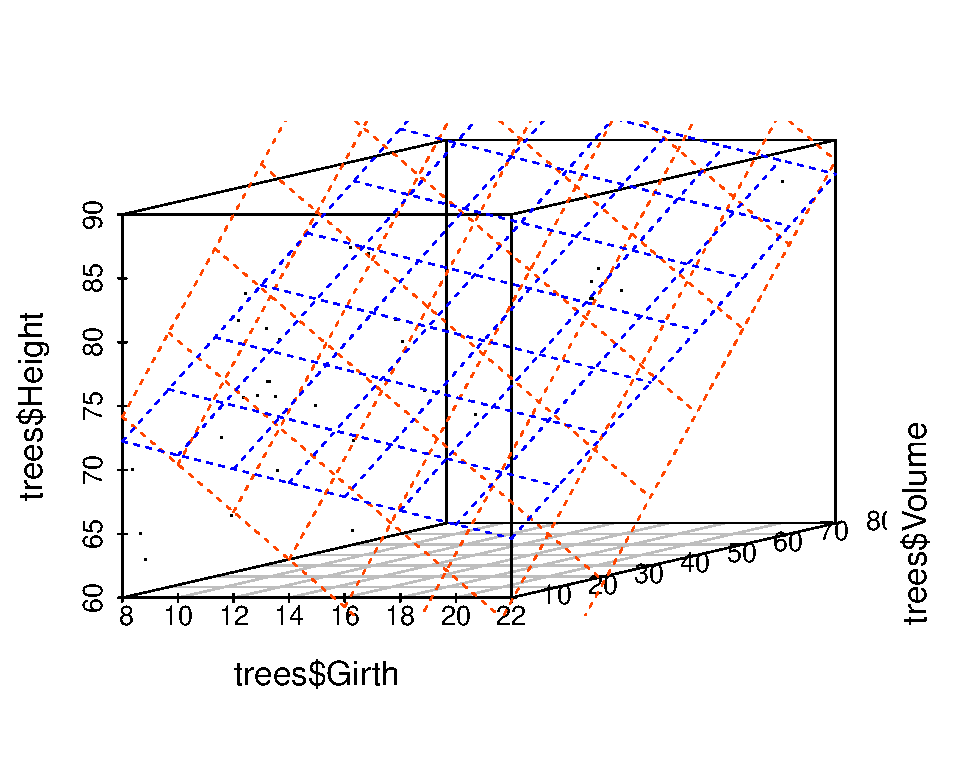
\includegraphics[width=0.5\columnwidth]{./figures/hands-on4/trees-jitterfit-height.pdf}
\caption{Multiple regression plot of cherry tree height on girth and volume, for the original data (red) and the jittered data (blue).\label{fig:jittercompare}}
\end{figure}



Let's do the same comparison for the multiple regression of Volume on Height and Girth.  In this case the predictor variables are \emph{not} nearly collinear.
%
\begin{R}
> lm.V <- lm(Volume ~ Girth + Height, data = trees)
> lm.V.jitter <- lm(Volume ~ Girth + Height, data = jitter.trees)
> coefficients(lm.V)
(Intercept)       Girth      Height 
-57.9876589   4.7081605   0.3392512 
> coefficients(lm.V.jitter)
(Intercept)       Girth      Height 
-51.2670818   4.4798268   0.2906203 
\end{R}
%
For this model, we see that the coefficients have changed only a small amount.  The underlying data, |jitter.trees|, is the same in both cases, but now our model is stable because the predictor variables are only modestly correlated with each other.

Let's generate another plot to illustrate the similarity of the models fit to the original and jittered data when Girth and Height are used to predict Volume. The corresponding output is shown in Fig.~\ref{fig:jittervolume}.
%
\begin{R}
> p <- scatterplot3d(x=trees$Girth, y=trees$Height, z=trees$Volume, 
                     angle=55, type='p', pch='.')
> p$plane3d(lm.V, col='orangered')
> p$plane3d(lm.V.jitter, col='blue')
\end{R}
%
\begin{figure}[htbp]
\centering
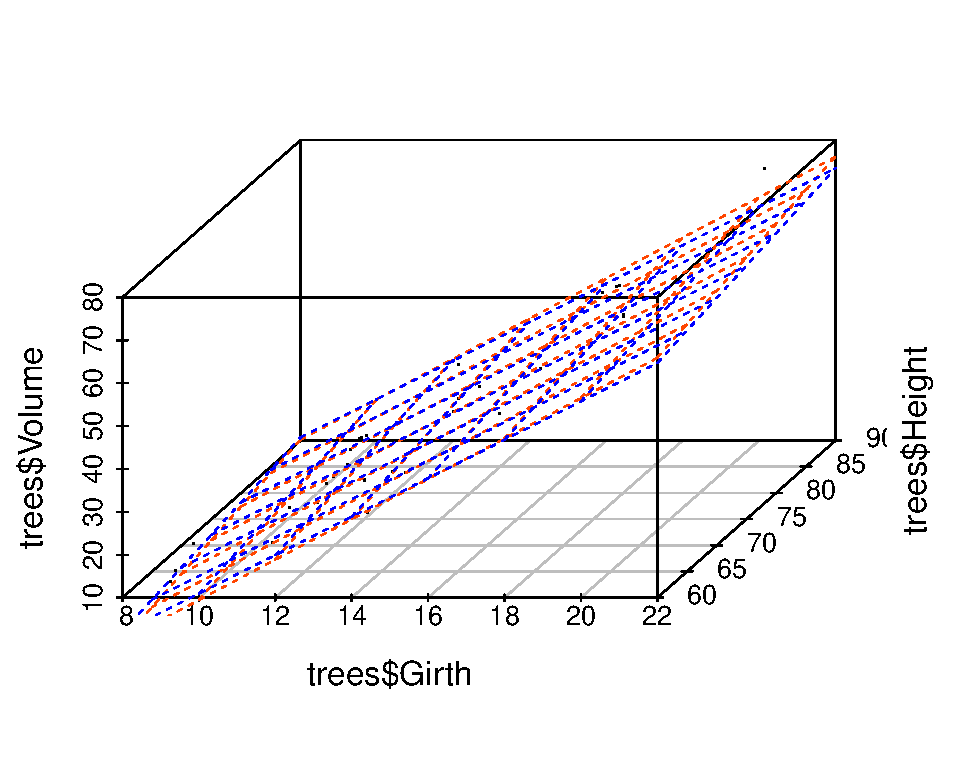
\includegraphics[width=0.5\columnwidth]{./figures/hands-on4/trees-jitterfit-volume.pdf}
\caption{Multiple regression plot of cherry tree volume on girth and height, for the original data (red) and the jittered data (blue).\label{fig:jittervolume}}
\end{figure}

Finally, let's do some vector calculations to quantify how the angular deviation between the fit data and the predictor variables changes between the original and jittered data set for the two different multiple regressions:
%
\begin{R}

# write a quickie fxn to express angle between vectors in degrees
> vec.angle <- function(x,y) { acos(cor(x,y)) * (180/pi)}

# vector angles for fit of Height ~ Girth + Volume (orig)
> vec.angle(lm.H$fitted.values, trees$Girth)
[1] 36.02644
> vec.angle(lm.H$fitted.values, trees$Volume)
[1] 21.29297

# vector angles for fit of Height ~ Girth + Volume (jittered)
> vec.angle(lm.H.jitter$fitted.values, jitter.trees$Girth)
[1] 28.48079
> vec.angle(lm.H.jitter$fitted.values, jitter.trees$Volume)
[1] 9.097828

# CONCLUSION -- angular changes of about 8 and 12 degrees 


# vector angles for fit of Volume ~ Girth + Height (orig)
> vec.angle(lm.V$fitted.values, trees$Girth)
[1] 6.628322
> vec.angle(lm.V$fitted.values, trees$Height)
[1] 52.08771

# vector angles for fit of Volume ~ Girth + Height (jittered)
> vec.angle(lm.V.jitter$fitted.values, jitter.trees$Girth)
[1] 6.163463
> vec.angle(lm.V.jitter$fitted.values, jitter.trees$Height)
[1] 54.33651

# CONCLUSION -- angular changes of about 0.5 and 2 degrees
\end{R}

\section{Manipulating data using split}

Last week we introduced the |reshape()| function from the reshape2 package.  |reshape()| is good for computing simple statistics across multiple `facets' of data. However, more complicated statistics are made possible by using the |split()| function, which is defined in the R base package.

|split()| takes two arguments: 1) a vector or data frame to split and 2) a character vector defining what to split the first argument by. For example, we can split the iris data set by species in order to get a list containing three data frames; one for each species.
%
\begin{R}
> iris.split <- split(iris, iris$Species)
> names(iris.split)
[1] "setosa"     "versicolor" "virginica" 
> str(iris.split)  # see the documentation for the str() function
List of 3
 $ setosa    :'data.frame': 50 obs. of  5 variables:
  ..$ Sepal.Length: num [1:50] 5.1 4.9 4.7 4.6 5 5.4 4.6 5 4.4 4.9 ...
  ..$ Sepal.Width : num [1:50] 3.5 3 3.2 3.1 3.6 3.9 3.4 3.4 2.9 3.1 ...
  ..$ Petal.Length: num [1:50] 1.4 1.4 1.3 1.5 1.4 1.7 1.4 1.5 1.4 1.5 ...
  ..$ Petal.Width : num [1:50] 0.2 0.2 0.2 0.2 0.2 0.4 0.3 0.2 0.2 0.1 ...
  ..$ Species     : Factor w/ 3 levels "setosa","versicolor",..: 1 1 1 1 1 1 1 1 1 1 ...
 $ versicolor:'data.frame': 50 obs. of  5 variables:
  ..$ Sepal.Length: num [1:50] 7 6.4 6.9 5.5 6.5 5.7 6.3 4.9 6.6 5.2 ...
  ..$ Sepal.Width : num [1:50] 3.2 3.2 3.1 2.3 2.8 2.8 3.3 2.4 2.9 2.7 ...
  ..$ Petal.Length: num [1:50] 4.7 4.5 4.9 4 4.6 4.5 4.7 3.3 4.6 3.9 ...
  ..$ Petal.Width : num [1:50] 1.4 1.5 1.5 1.3 1.5 1.3 1.6 1 1.3 1.4 ...
  ..$ Species     : Factor w/ 3 levels "setosa","versicolor",..: 2 2 2 2 2 2 2 2 2 2 ...
 $ virginica :'data.frame': 50 obs. of  5 variables:
  ..$ Sepal.Length: num [1:50] 6.3 5.8 7.1 6.3 6.5 7.6 4.9 7.3 6.7 7.2 ...
  ..$ Sepal.Width : num [1:50] 3.3 2.7 3 2.9 3 3 2.5 2.9 2.5 3.6 ...
  ..$ Petal.Length: num [1:50] 6 5.1 5.9 5.6 5.8 6.6 4.5 6.3 5.8 6.1 ...
  ..$ Petal.Width : num [1:50] 2.5 1.9 2.1 1.8 2.2 2.1 1.7 1.8 1.8 2.5 ...
  ..$ Species     : Factor w/ 3 levels "setosa","versicolor",..: 3 3 3 3 3 3 3 3 3 3 ...
\end{R}

Now that we have a split data frame, it's easy to use |lapply| or |sapply| to calculate complicated summary statistics. For example, this function calculates the mean ratio of |Sepal.Length| to |Petal.Length|:
%
\begin{R}
> ratio.sepal2petal <- function(x) {
+    mean( x$Sepal.Length / x$Petal.Length)
+ }
> sapply(iris.split, ratio.sepal2petal)
    setosa versicolor  virginica 
  3.464906   1.400896   1.188350 
\end{R}
%
We could also write a function to return the coefficients of fitting a linear model to each facet of the data:
%
\begin{R}
> sepal.on.petal.coeff <- function(x){
+       model <- lm(Sepal.Length ~ Petal.Length, data=x)
+       return(model$coeff)
+ }
> sapply(iris.split, sepal.on.petal.coeff)
                setosa versicolor virginica
(Intercept)  4.2131682   2.407523 1.0596591
Petal.Length 0.5422926   0.828281 0.9957386
\end{R}
%
Of course, no analysis would be complete without examining the fit of the linear models. In order to visualize whether the linear model is a good representation of the data, we'll write another function to return a data frame containing the fitted values, residuals, and species names for each element of the list.
%
\begin{R}
> sepal.on.petal.lm.fit <- function(x){
+       model <- lm(Sepal.Length ~ Petal.Length, data=x)
+       data.frame(fitted = fitted(model),
+                  residuals = residuals(model),
+                  species = x$Species)
+ }
> iris.fit <- lapply(iris.split, sepal.on.petal.lm.fit)
> str(iris.fit)
List of 3
 $ setosa    :'data.frame': 50 obs. of  3 variables:
  ..$ fitted   : num [1:50] 4.97 4.97 4.92 5.03 4.97 ...
  ..$ residuals: num [1:50] 0.1276 -0.0724 -0.2181 -0.4266 0.0276 ...
  ..$ species  : Factor w/ 3 levels "setosa","versicolor",..: 1 1 1 1 1 1 1 1 1 1 ...
 $ versicolor:'data.frame': 50 obs. of  3 variables:
  ..$ fitted   : num [1:50] 6.3 6.13 6.47 5.72 6.22 ...
  ..$ residuals: num [1:50] 0.7 0.265 0.434 -0.221 0.282 ...
  ..$ species  : Factor w/ 3 levels "setosa","versicolor",..: 2 2 2 2 2 2 2 2 2 2 ...
 $ virginica :'data.frame': 50 obs. of  3 variables:
  ..$ fitted   : num [1:50] 7.03 6.14 6.93 6.64 6.83 ...
  ..$ residuals: num [1:50] -0.734 -0.338 0.165 -0.336 -0.335 ...
  ..$ species  : Factor w/ 3 levels "setosa","versicolor",..: 3 3 3 3 3 3 3 3 3 3 ...
> 
\end{R}

Next, we'll join the data back into a data frame using the |do.call| and |rbind| functions. Read the documentation to figure out what they do.
%
\begin{R}
> iris.joined <- do.call('rbind', iris.fit)
> str(iris.joined)
'data.frame': 150 obs. of  3 variables:
 $ fitted   : num  4.97 4.97 4.92 5.03 4.97 ...
 $ residuals: num  0.1276 -0.0724 -0.2181 -0.4266 0.0276 ...
 $ species  : Factor w/ 3 levels "setosa","versicolor",..: 1 1 1 1 1 1 1 1 1 1 ...
\end{R}

Finally, we'll visualize our model fits by plotting our data using ggplot:
%
\begin{R}
> library(ggplot2)
> ggplot(iris.joined, aes(x=fitted, y=residuals))+
+   geom_point()+
+   facet_wrap(~species, scale='free') + 
+   ggtitle("Residuals from Regression of \nSepal Length on Petal Length for 3 Iris Species")
\end{R}
Examining the residuals (Fig.~\ref{fig:irissplit}), we see they look fairly uniform across the range of fit values. The term that statiscians use for this is `homoscedastic'; when the residuals are non uniform we say they are `heteroscadistic'.
%
\begin{figure}[htbp]
\centering
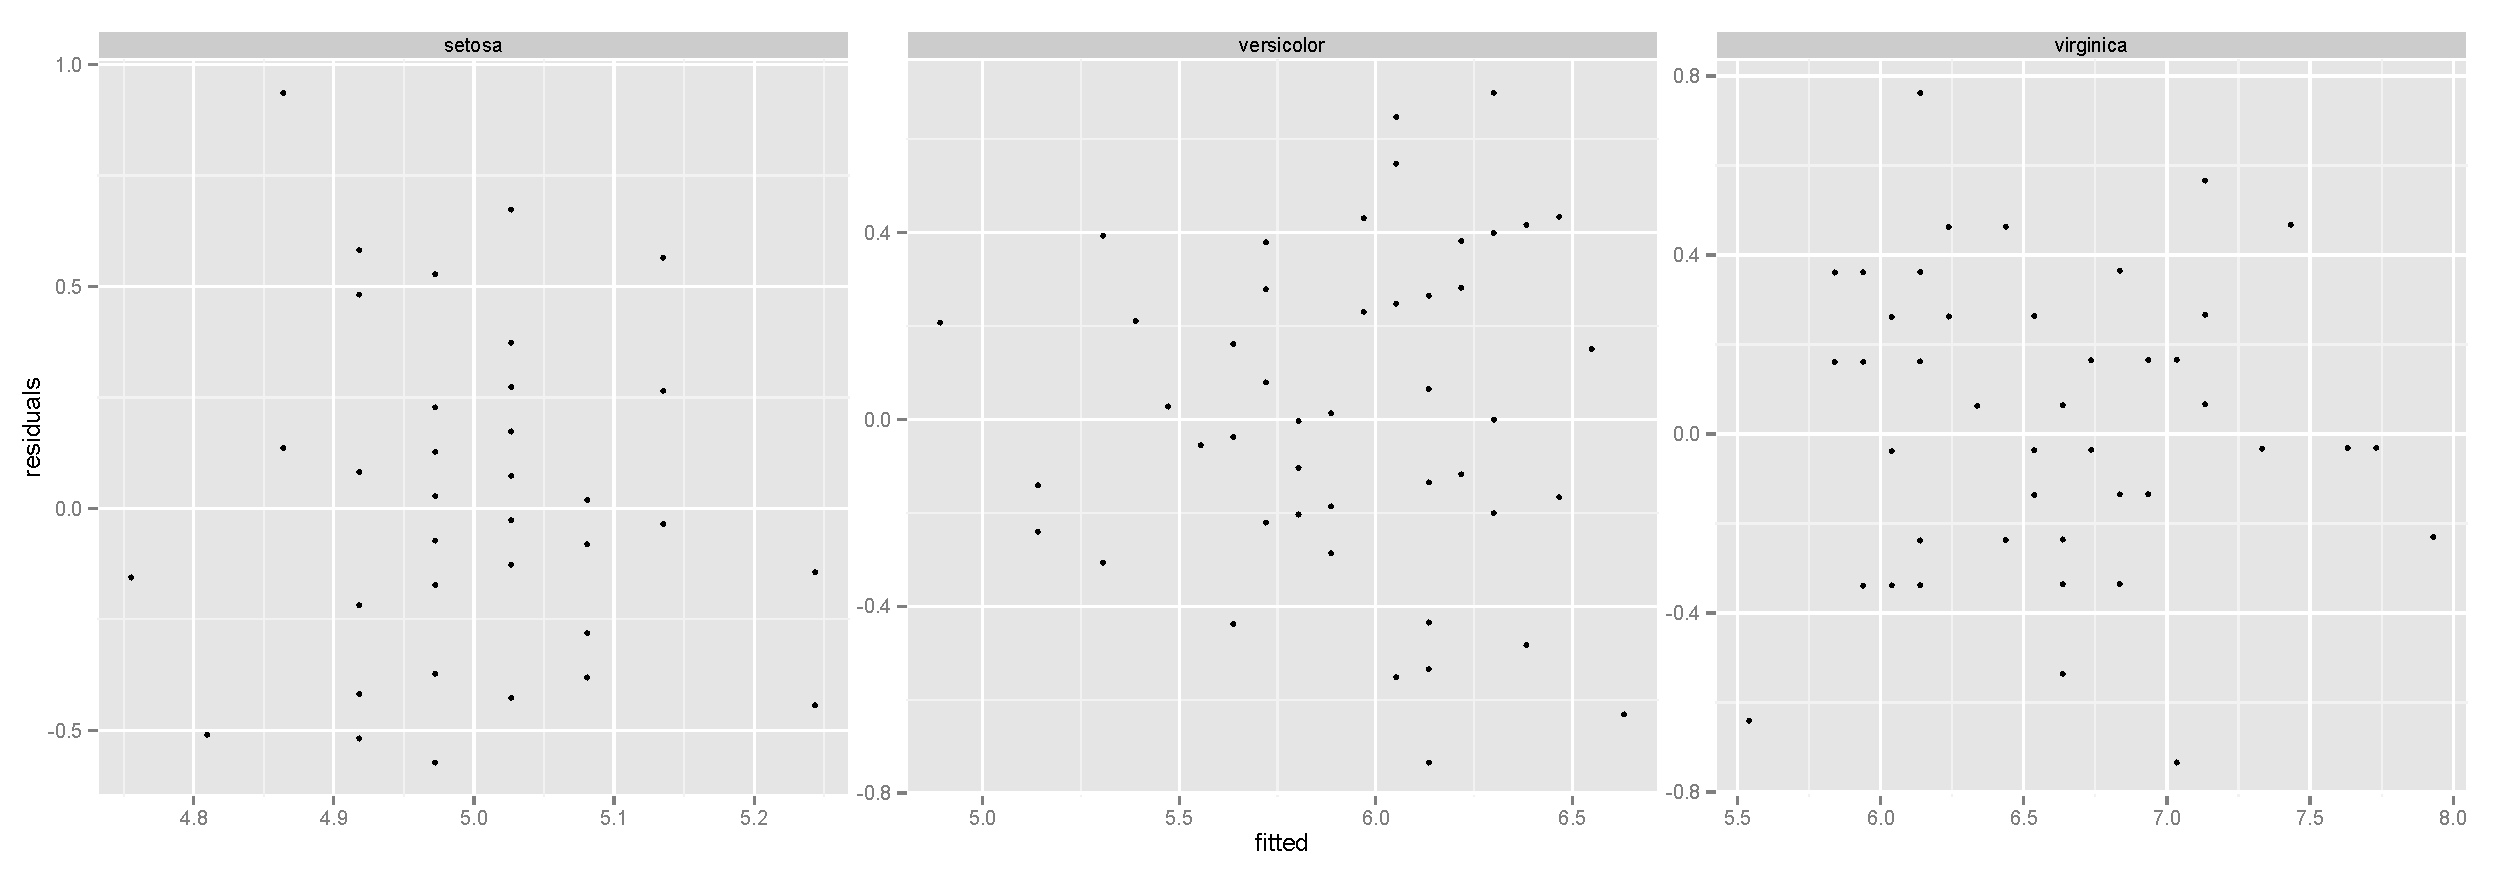
\includegraphics[width=0.75\columnwidth]{./figures/hands-on4/iris-residuals.pdf}
\caption{Residuals from regressions of Sepal Length on Petal Length, for the Iris data set split by species.\label{fig:irissplit}}
\end{figure}


An alternate way to visualize the fits, without the benefit of  getting the info on the model fits back for further examination, is to use the |stat_smooth()| to plot a linear fit of our data for each facet (Fig.~\ref{fig:irisregressions}). Read the |stat_smooth| documentation to how this works.
%
\begin{R}
> ggplot( iris, aes(x=Petal.Length, y=Sepal.Length))+
   geom_point()+
   stat_smooth(method="lm")+
   facet_wrap(~Species, scale='free')+
   ggtitle("Regressions of Sepal Length on Petal Length")
\end{R}
%
\begin{figure}[htbp]
\centering
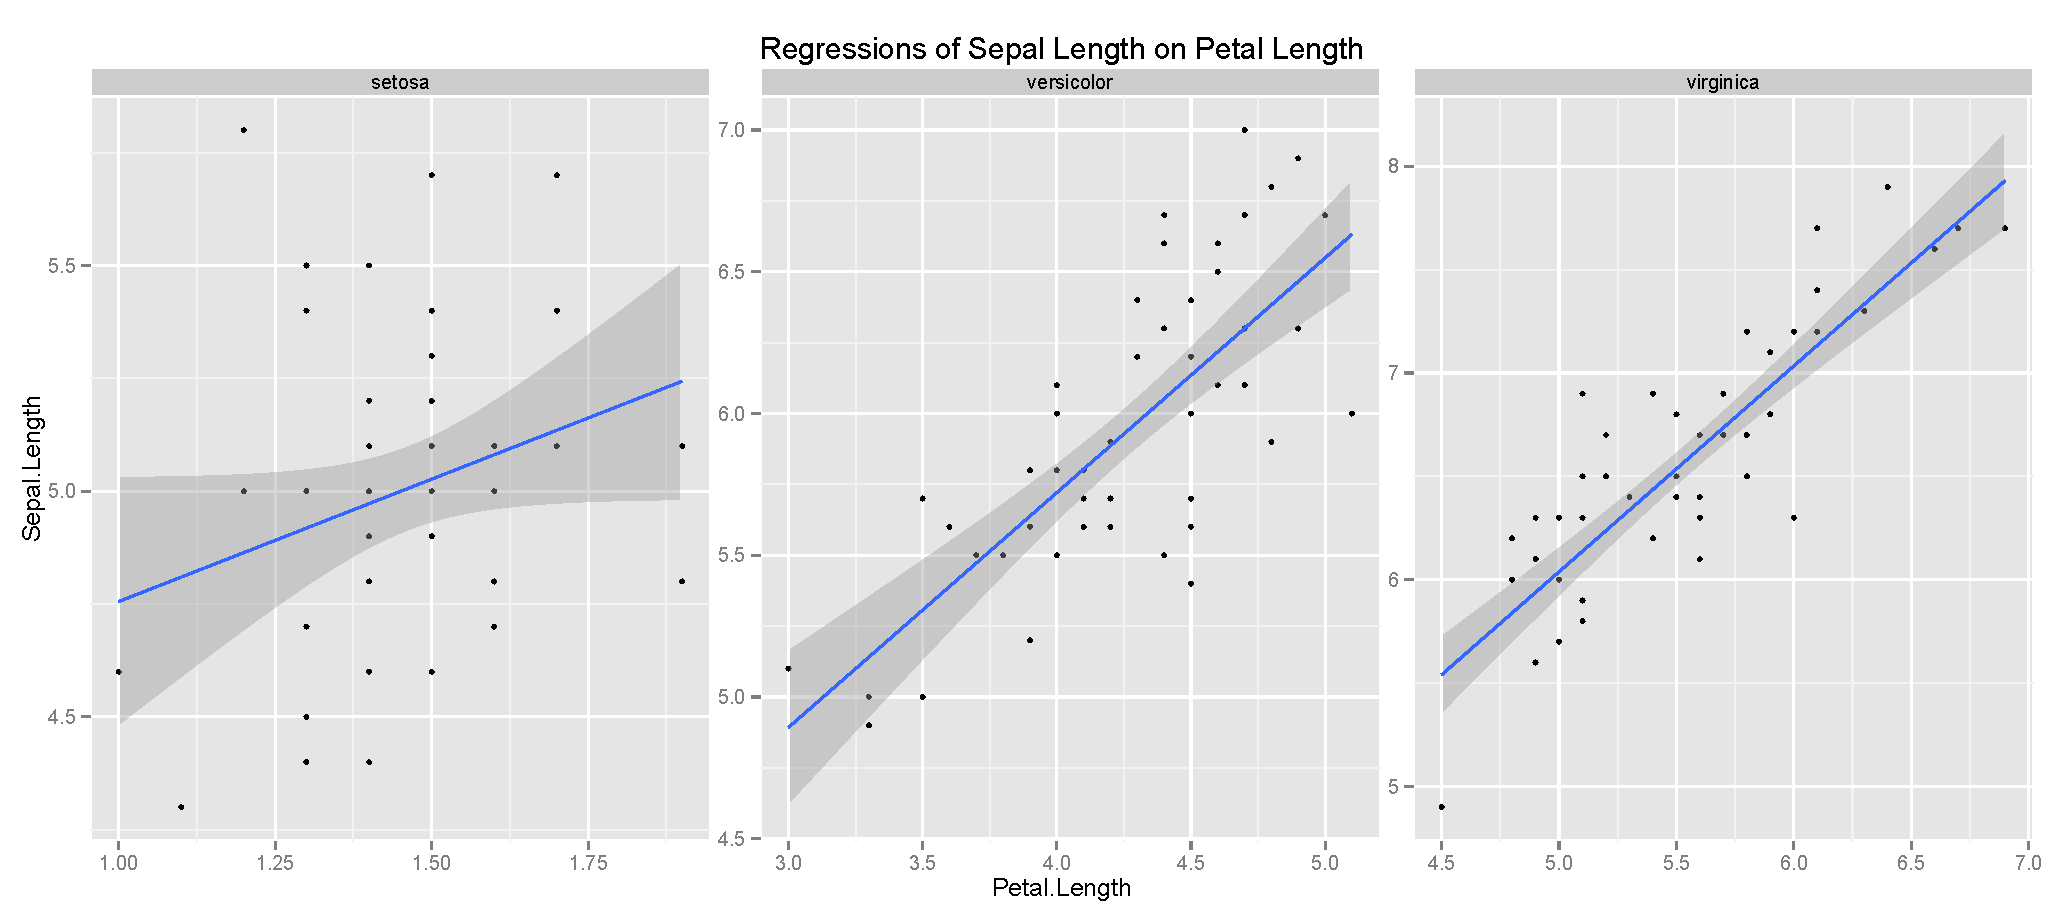
\includegraphics[width=0.75\columnwidth]{./figures/hands-on4/iris-regressions.pdf}
\caption{Regressions of Sepal Length on Petal Length, for the Iris data, produced using the \lstinline|stat_smooth()| function in ggplot2.\label{fig:irisregressions}}
\end{figure}
%



\end{document}

